% Options for packages loaded elsewhere
\PassOptionsToPackage{unicode}{hyperref}
\PassOptionsToPackage{hyphens}{url}
%
\documentclass[
  ignorenonframetext,
]{beamer}
\usepackage{pgfpages}
\setbeamertemplate{caption}[numbered]
\setbeamertemplate{caption label separator}{: }
\setbeamercolor{caption name}{fg=normal text.fg}
\beamertemplatenavigationsymbolsempty
% Prevent slide breaks in the middle of a paragraph
\widowpenalties 1 10000
\raggedbottom
\setbeamertemplate{part page}{
  \centering
  \begin{beamercolorbox}[sep=16pt,center]{part title}
    \usebeamerfont{part title}\insertpart\par
  \end{beamercolorbox}
}
\setbeamertemplate{section page}{
  \centering
  \begin{beamercolorbox}[sep=12pt,center]{part title}
    \usebeamerfont{section title}\insertsection\par
  \end{beamercolorbox}
}
\setbeamertemplate{subsection page}{
  \centering
  \begin{beamercolorbox}[sep=8pt,center]{part title}
    \usebeamerfont{subsection title}\insertsubsection\par
  \end{beamercolorbox}
}
\AtBeginPart{
  \frame{\partpage}
}
\AtBeginSection{
  \ifbibliography
  \else
    \frame{\sectionpage}
  \fi
}
\AtBeginSubsection{
  \frame{\subsectionpage}
}
\usepackage{amsmath,amssymb}
\usepackage{lmodern}
\usepackage{iftex}
\ifPDFTeX
  \usepackage[T1]{fontenc}
  \usepackage[utf8]{inputenc}
  \usepackage{textcomp} % provide euro and other symbols
\else % if luatex or xetex
  \usepackage{unicode-math}
  \defaultfontfeatures{Scale=MatchLowercase}
  \defaultfontfeatures[\rmfamily]{Ligatures=TeX,Scale=1}
\fi
% Use upquote if available, for straight quotes in verbatim environments
\IfFileExists{upquote.sty}{\usepackage{upquote}}{}
\IfFileExists{microtype.sty}{% use microtype if available
  \usepackage[]{microtype}
  \UseMicrotypeSet[protrusion]{basicmath} % disable protrusion for tt fonts
}{}
\makeatletter
\@ifundefined{KOMAClassName}{% if non-KOMA class
  \IfFileExists{parskip.sty}{%
    \usepackage{parskip}
  }{% else
    \setlength{\parindent}{0pt}
    \setlength{\parskip}{6pt plus 2pt minus 1pt}}
}{% if KOMA class
  \KOMAoptions{parskip=half}}
\makeatother
\usepackage{xcolor}
\newif\ifbibliography
\usepackage{color}
\usepackage{fancyvrb}
\newcommand{\VerbBar}{|}
\newcommand{\VERB}{\Verb[commandchars=\\\{\}]}
\DefineVerbatimEnvironment{Highlighting}{Verbatim}{commandchars=\\\{\}}
% Add ',fontsize=\small' for more characters per line
\usepackage{framed}
\definecolor{shadecolor}{RGB}{248,248,248}
\newenvironment{Shaded}{\begin{snugshade}}{\end{snugshade}}
\newcommand{\AlertTok}[1]{\textcolor[rgb]{0.94,0.16,0.16}{#1}}
\newcommand{\AnnotationTok}[1]{\textcolor[rgb]{0.56,0.35,0.01}{\textbf{\textit{#1}}}}
\newcommand{\AttributeTok}[1]{\textcolor[rgb]{0.77,0.63,0.00}{#1}}
\newcommand{\BaseNTok}[1]{\textcolor[rgb]{0.00,0.00,0.81}{#1}}
\newcommand{\BuiltInTok}[1]{#1}
\newcommand{\CharTok}[1]{\textcolor[rgb]{0.31,0.60,0.02}{#1}}
\newcommand{\CommentTok}[1]{\textcolor[rgb]{0.56,0.35,0.01}{\textit{#1}}}
\newcommand{\CommentVarTok}[1]{\textcolor[rgb]{0.56,0.35,0.01}{\textbf{\textit{#1}}}}
\newcommand{\ConstantTok}[1]{\textcolor[rgb]{0.00,0.00,0.00}{#1}}
\newcommand{\ControlFlowTok}[1]{\textcolor[rgb]{0.13,0.29,0.53}{\textbf{#1}}}
\newcommand{\DataTypeTok}[1]{\textcolor[rgb]{0.13,0.29,0.53}{#1}}
\newcommand{\DecValTok}[1]{\textcolor[rgb]{0.00,0.00,0.81}{#1}}
\newcommand{\DocumentationTok}[1]{\textcolor[rgb]{0.56,0.35,0.01}{\textbf{\textit{#1}}}}
\newcommand{\ErrorTok}[1]{\textcolor[rgb]{0.64,0.00,0.00}{\textbf{#1}}}
\newcommand{\ExtensionTok}[1]{#1}
\newcommand{\FloatTok}[1]{\textcolor[rgb]{0.00,0.00,0.81}{#1}}
\newcommand{\FunctionTok}[1]{\textcolor[rgb]{0.00,0.00,0.00}{#1}}
\newcommand{\ImportTok}[1]{#1}
\newcommand{\InformationTok}[1]{\textcolor[rgb]{0.56,0.35,0.01}{\textbf{\textit{#1}}}}
\newcommand{\KeywordTok}[1]{\textcolor[rgb]{0.13,0.29,0.53}{\textbf{#1}}}
\newcommand{\NormalTok}[1]{#1}
\newcommand{\OperatorTok}[1]{\textcolor[rgb]{0.81,0.36,0.00}{\textbf{#1}}}
\newcommand{\OtherTok}[1]{\textcolor[rgb]{0.56,0.35,0.01}{#1}}
\newcommand{\PreprocessorTok}[1]{\textcolor[rgb]{0.56,0.35,0.01}{\textit{#1}}}
\newcommand{\RegionMarkerTok}[1]{#1}
\newcommand{\SpecialCharTok}[1]{\textcolor[rgb]{0.00,0.00,0.00}{#1}}
\newcommand{\SpecialStringTok}[1]{\textcolor[rgb]{0.31,0.60,0.02}{#1}}
\newcommand{\StringTok}[1]{\textcolor[rgb]{0.31,0.60,0.02}{#1}}
\newcommand{\VariableTok}[1]{\textcolor[rgb]{0.00,0.00,0.00}{#1}}
\newcommand{\VerbatimStringTok}[1]{\textcolor[rgb]{0.31,0.60,0.02}{#1}}
\newcommand{\WarningTok}[1]{\textcolor[rgb]{0.56,0.35,0.01}{\textbf{\textit{#1}}}}
\usepackage{longtable,booktabs,array}
\usepackage{calc} % for calculating minipage widths
\usepackage{caption}
% Make caption package work with longtable
\makeatletter
\def\fnum@table{\tablename~\thetable}
\makeatother
\usepackage{graphicx}
\makeatletter
\def\maxwidth{\ifdim\Gin@nat@width>\linewidth\linewidth\else\Gin@nat@width\fi}
\def\maxheight{\ifdim\Gin@nat@height>\textheight\textheight\else\Gin@nat@height\fi}
\makeatother
% Scale images if necessary, so that they will not overflow the page
% margins by default, and it is still possible to overwrite the defaults
% using explicit options in \includegraphics[width, height, ...]{}
\setkeys{Gin}{width=\maxwidth,height=\maxheight,keepaspectratio}
% Set default figure placement to htbp
\makeatletter
\def\fps@figure{htbp}
\makeatother
\setlength{\emergencystretch}{3em} % prevent overfull lines
\providecommand{\tightlist}{%
  \setlength{\itemsep}{0pt}\setlength{\parskip}{0pt}}
\setcounter{secnumdepth}{-\maxdimen} % remove section numbering
\ifLuaTeX
  \usepackage{selnolig}  % disable illegal ligatures
\fi
\IfFileExists{bookmark.sty}{\usepackage{bookmark}}{\usepackage{hyperref}}
\IfFileExists{xurl.sty}{\usepackage{xurl}}{} % add URL line breaks if available
\urlstyle{same} % disable monospaced font for URLs
\hypersetup{
  pdftitle={MQE: Economic Inference from Data: Module 5: Difference in Differences},
  pdfauthor={Claire Duquennois},
  hidelinks,
  pdfcreator={LaTeX via pandoc}}

\title{MQE: Economic Inference from Data:\\
Module 5: Difference in Differences}
\author{Claire Duquennois}
\date{6/9/2020}

\begin{document}
\frame{\titlepage}

\begin{frame}{Causal Inference with non-random assignment:}
\protect\hypertarget{causal-inference-with-non-random-assignment}{}
Randomizing treatment is not always possible:

\begin{itemize}
\item
  the program or policy has already happened
\item
  randomization in unfeasible
\item
  randomizing treatment would be unethical (ex: randomizing exposure to
  pollutants)
\end{itemize}
\end{frame}

\begin{frame}{Causal Inference with non-random assignment:}
\protect\hypertarget{causal-inference-with-non-random-assignment-1}{}
With no randomized control trial we have to assume that the treatment
was not randomly assigned:

\begin{itemize}
\item
  treatment will depend on observable and/or unobservable
  characteristics
\item
  their are important differences between our treated and untreated
  units that we cannot control for
\item
  Leaving these variables out in the error term will cause OVB.
\end{itemize}

Differences-in-differences is a way of getting around non-random
assignment of a treatment.
\end{frame}

\begin{frame}{DID: Example and intuition\footnote<.->{This section is
  borrowed from scunning.com}}
\protect\hypertarget{did-example-and-intuition}{}
2002: Craigslist opens a new section called ``erotic services'' in San
Francisco:

\begin{itemize}
\item
  mostly used by sex workers to advertise and solicit clients.
\item
  Sex workers claimed it made them safer, because they could solicit
  indoors from their computers and learn more about the men contacting
  them.
\item
  Activists and law enforcement worried that it was facilitating sex
  trafficking and increasing violence against women.
\end{itemize}

Which was it? Was erotic services (ERS) making women safer, or was it
placing them in harm's way?
\end{frame}

\begin{frame}{SOS Empiricist!}
\protect\hypertarget{sos-empiricist}{}
This is an empirical question: What is the effect of ERS on female
safety?

\begin{itemize}
\item
  The fundamental problem of causal inference strikes again!
\item
  We can't know what effect it had because we are missing the data for
  the counterfactual:
\end{itemize}

\[
E[\tau]=E[\underbrace{Y_{SF,2003}(D_{SF,2003}=1)}_\text{observed}]-E[\underbrace{Y_{SF,2003}(D_{SF,2003}=0)}_\text{unobserved}]
\]

In 2003 only the first occurs, and the second is a counterfactual. So
how do we proceed?
\end{frame}

\begin{frame}{Diff-in-Diff to the rescue:}
\protect\hypertarget{diff-in-diff-to-the-rescue}{}
The standard differences-in-differences strategy (DiD):

\begin{itemize}
\item
  Define the intervention, \(D\)= the availability of the Craigslist ERS
  webpage.
\item
  We want to know the causal effect, \(\tau\) of \(D\) on \(Y\)= female
  murders.
\end{itemize}

Can we just compare SF murders in, say, 2003 with some other city, like
Pittsburgh?
\end{frame}

\begin{frame}{Differencing A:}
\protect\hypertarget{differencing-a}{}
\begin{longtable}[]{@{}ll@{}}
\toprule()
\ldots.City\ldots. &
\ldots\ldots\ldots..Outcome\ldots\ldots\ldots\ldots. \\
\midrule()
\endhead
San Francisco & \(Y_{SF,2003}=\alpha_{SF}+\tau\) \\
Pittsburgh & \(Y_{P,2003}=\alpha_{P}\) \\
\bottomrule()
\end{longtable}

\begin{itemize}
\item
  \(\alpha_{SF}\) is a San Francisco fixed effect
\item
  \(\alpha_P\) is a Pittsburgh fixed effect.
\end{itemize}

If make a simple comparison between Pittsburgh and SF:

\[
\tilde{\tau}=Y_{SF,2003}-Y_{P,2003}=\alpha_{SF}+\tau-\alpha_{P}.
\]
\end{frame}

\begin{frame}{Differencing A:}
\protect\hypertarget{differencing-a-1}{}
The simple difference is biased because of the difference in the
underlying murder rates between the two cities:

\[
\tilde{\tau}-\tau=\alpha_{SF}-\alpha_{P}. 
\]
\end{frame}

\begin{frame}{Differencing B:}
\protect\hypertarget{differencing-b}{}
What if we compare SF to itself? Say in 2003 to 2001?

\begin{longtable}[]{@{}ccc@{}}
\toprule()
\ldots..City\ldots. & ..Time.. &
\ldots\ldots\ldots.Outcome\ldots\ldots\ldots\ldots. \\
\midrule()
\endhead
San Francisco & Before & \(Y_{SF,2001}=\alpha_{SF}\) \\
& After & \(Y_{SF,2003}=\alpha_{SF}+\lambda_{03}+\tau\) \\
\bottomrule()
\end{longtable}

Again, this doesn't lead to an unbiased estimate of \(\tau\) since: \[
\tilde{\tau}=\alpha_{SF}+\lambda_{03}+\tau-\alpha_{SF}=\lambda_{03}+\tau
\]

We eliminated the city fixed effect but not the changes in the murder
rate over time which will bias my estimate: \[
\tilde{\tau}-\tau=\lambda_{03}
\] \textbf{How can I identify and control for these time effects?}
\end{frame}

\begin{frame}{Differencing A+B= Diff-in-Diff}
\protect\hypertarget{differencing-ab-diff-in-diff}{}
Combining the two approaches to eliminate both the city effects and the
time effects:

\begin{longtable}[]{@{}
  >{\raggedright\arraybackslash}p{(\columnwidth - 8\tabcolsep) * \real{0.1512}}
  >{\raggedright\arraybackslash}p{(\columnwidth - 8\tabcolsep) * \real{0.0465}}
  >{\raggedright\arraybackslash}p{(\columnwidth - 8\tabcolsep) * \real{0.4535}}
  >{\raggedright\arraybackslash}p{(\columnwidth - 8\tabcolsep) * \real{0.1860}}
  >{\raggedright\arraybackslash}p{(\columnwidth - 8\tabcolsep) * \real{0.1628}}@{}}
\toprule()
\begin{minipage}[b]{\linewidth}\raggedright
\ldots City\ldots{}
\end{minipage} & \begin{minipage}[b]{\linewidth}\raggedright
..Time..
\end{minipage} & \begin{minipage}[b]{\linewidth}\raggedright
\ldots\ldots..Outcome\ldots\ldots..
\end{minipage} & \begin{minipage}[b]{\linewidth}\raggedright
1st Diff
\end{minipage} & \begin{minipage}[b]{\linewidth}\raggedright
2nd Diff
\end{minipage} \\
\midrule()
\endhead
SF & Before & \(Y_{SF,2001}=\alpha_{SF}\) & & \\
& After & \(Y_{SF,2003}=\alpha_{SF}+\lambda_{03}+\tau\) &
\(\lambda_{03}+\tau\) & \\
& & & & \(\tau\) \\
Pittsburgh & Before & \(Y_{P,2001}=\alpha_{P}\) & & \\
& After & \(Y_{P,2003}=\alpha_{P}+\lambda_{03}\) & \(\lambda_{03}\) & \\
\bottomrule()
\end{longtable}
\end{frame}

\begin{frame}{The idea}
\protect\hypertarget{the-idea}{}
Sometimes treatment and control group outcomes move in parallel in the
absence of treatment.

When they do, the divergence of a post-treatment path from the trend
established by a comparison group may signal a treatment effect.
\end{frame}

\begin{frame}{The mechanics}
\protect\hypertarget{the-mechanics}{}
Difference-in-differences can be implemented as follows:

\begin{enumerate}
[1)]
\tightlist
\item
  Compute the difference in the mean outcome variable \(Y\) in the post
  treatment period \((t=1)\) and the before treatment period \((t=0)\)
  for the control group \(C\):
\end{enumerate}

\[
\bar{Y}_{C,1}-\bar{Y}_{C,0}=\Delta \bar{Y}_C
\]

\(\Rightarrow\) allows us to cancel out the control group fixed effect
and identify the time fixed effect since \[
\bar{Y}_{C,1}-\bar{Y}_{C,0}=\alpha_C+\lambda_1-\alpha_C=\lambda_1=\Delta \bar{Y}_C
\]
\end{frame}

\begin{frame}{The mechanics}
\protect\hypertarget{the-mechanics-1}{}
\begin{enumerate}
[1)]
\setcounter{enumi}{1}
\tightlist
\item
  Compute the difference in the mean outcome variable \(Y\) in the post
  treatment period \((t=1)\) and the before treatment period \((t=0)\)
  for the treated group \(T\):
\end{enumerate}

\[
\bar{Y}_{T,1}-\bar{Y}_{T,0}=\Delta \bar{Y}_T
\] which allows us to cancel out the treated group fixed effect \[
\bar{Y}_{T,1}-\bar{Y}_{T,0}=\alpha_T+\lambda_1+\tau-\alpha_T=\lambda_1+\tau=\Delta \bar{Y}_T
\]
\end{frame}

\begin{frame}{The mechanics}
\protect\hypertarget{the-mechanics-2}{}
\begin{enumerate}
[1)]
\setcounter{enumi}{2}
\tightlist
\item
  Treatment impact is then measured by the difference-in-differences:
\end{enumerate}

\[
(\bar{Y}_{T,1}-\bar{Y}_{T,0})-(\bar{Y}_{C,1}-\bar{Y}_{C,0})=(\Delta \bar{Y}_T-\Delta \bar{Y}_C)
\] since by comparing the differences we can cancel out the time fixed
effect and isolate the treatment effect of interest:

\[
\Delta \bar{Y}_T-\Delta \bar{Y}_C=\lambda_1+\tau-\lambda_1=\tau
\]
\end{frame}

\begin{frame}{DID Regressions:}
\protect\hypertarget{did-regressions}{}
This can be done in a regression framework:

\textbf{How would you specify this regression?}

\(\Rightarrow\) Top Hat
\end{frame}

\begin{frame}{DID Regressions:}
\protect\hypertarget{did-regressions-1}{}
This can be done in a regression framework:

\[
Y_{it}=\beta_0+\beta_1 Post_t+\beta_2 GetsTreat_i+\beta_3 Post_t\times GetsTreat_i+u_{it}
\]

\begin{itemize}
\item
  \(Post_t\) is an indicator for the post treatment period,
\item
  \(GetsTreat_i\) is an indicator for observations in the treatment
  group that eventually gets treated.
\end{itemize}

\textbf{Which coefficient identifies the treatment effect?}

\(\Rightarrow\) Top Hat
\end{frame}

\begin{frame}{DID Regressions:}
\protect\hypertarget{did-regressions-2}{}
\(\beta_3\) is the difference-in-differences estimator:

\begin{itemize}
\tightlist
\item
  estimates the differential impact of being in the post treatment
  period if you are in the treated group since
\end{itemize}

\small

\[
\begin{aligned}
E[Y_{C,1}]-E[Y_{C,0}]&=(\beta_0+\beta_1)-(\beta_0)=\beta_1\\
E[Y_{T,1}]-E[Y_{T,0}]&=(\beta_0+\beta_1+\beta_2+\beta_3)-(\beta_0+\beta_2)=\beta_1+\beta_3\\
\end{aligned}
\]

\[
(E[Y_{T,1}]-E[Y_{T,0}])-(E[Y_{C,1}]-E[Y_{C,0}])=\beta_3
\]
\end{frame}

\begin{frame}{A simulation:}
\protect\hypertarget{a-simulation}{}
Suppose you are a principal of a school:

\begin{itemize}
\item
  ten 4th grade classrooms of 30 students each.
\item
  Starting in 2001 school year, teachers can enroll their class in the
  scholastic book club
\item
  4 of your fourth grade teachers opted to enroll.
\end{itemize}

You are interested in estimating the effect of participation in the book
club on 4th grade reading scores.
\end{frame}

\begin{frame}[fragile]{A simulation:}
\protect\hypertarget{a-simulation-1}{}
\tiny

\begin{Shaded}
\begin{Highlighting}[]
\FunctionTok{set.seed}\NormalTok{(}\DecValTok{6000}\NormalTok{)}
\NormalTok{scores }\OtherTok{\textless{}{-}} \FunctionTok{as.data.frame}\NormalTok{(}\FunctionTok{rep}\NormalTok{(}\FunctionTok{c}\NormalTok{(}\DecValTok{1}\NormalTok{, }\DecValTok{2}\NormalTok{, }\DecValTok{3}\NormalTok{, }\DecValTok{4}\NormalTok{, }\DecValTok{5}\NormalTok{, }\DecValTok{6}\NormalTok{, }\DecValTok{7}\NormalTok{, }\DecValTok{8}\NormalTok{, }\DecValTok{9}\NormalTok{, }\DecValTok{10}\NormalTok{),}
    \AttributeTok{times =} \DecValTok{30}\NormalTok{))}
\FunctionTok{names}\NormalTok{(scores) }\OtherTok{\textless{}{-}} \FunctionTok{c}\NormalTok{(}\StringTok{"class"}\NormalTok{)}
\NormalTok{scores }\OtherTok{\textless{}{-}}\NormalTok{ fastDummies}\SpecialCharTok{::}\FunctionTok{dummy\_cols}\NormalTok{(scores, }\AttributeTok{select\_columns =} \StringTok{"class"}\NormalTok{)}

\NormalTok{scores}\SpecialCharTok{$}\NormalTok{error }\OtherTok{\textless{}{-}} \FunctionTok{rnorm}\NormalTok{(}\DecValTok{300}\NormalTok{, }\AttributeTok{mean =} \DecValTok{0}\NormalTok{, }\AttributeTok{sd =} \DecValTok{10}\NormalTok{)}

\CommentTok{\# suppose teachers in the better performing classes}
\CommentTok{\# (classes, 7,8,9,10) select to participate in the book}
\CommentTok{\# club program}
\NormalTok{scores}\SpecialCharTok{$}\NormalTok{treat }\OtherTok{\textless{}{-}} \DecValTok{0}
\NormalTok{scores}\SpecialCharTok{$}\NormalTok{treat[scores}\SpecialCharTok{$}\NormalTok{class }\SpecialCharTok{\%in\%} \FunctionTok{c}\NormalTok{(}\DecValTok{7}\NormalTok{, }\DecValTok{8}\NormalTok{, }\DecValTok{9}\NormalTok{, }\DecValTok{10}\NormalTok{)] }\OtherTok{\textless{}{-}} \DecValTok{1}

\NormalTok{tau }\OtherTok{\textless{}{-}} \DecValTok{10}

\CommentTok{\# the data generating process}
\NormalTok{scores}\SpecialCharTok{$}\NormalTok{read4 }\OtherTok{\textless{}{-}}\NormalTok{ (}\DecValTok{85} \SpecialCharTok{+}\NormalTok{ tau }\SpecialCharTok{*}\NormalTok{ scores}\SpecialCharTok{$}\NormalTok{treat }\SpecialCharTok{+}\NormalTok{ (}\SpecialCharTok{{-}}\DecValTok{10}\NormalTok{) }\SpecialCharTok{*}\NormalTok{ scores}\SpecialCharTok{$}\NormalTok{class\_1 }\SpecialCharTok{+}
\NormalTok{    (}\SpecialCharTok{{-}}\DecValTok{15}\NormalTok{) }\SpecialCharTok{*}\NormalTok{ scores}\SpecialCharTok{$}\NormalTok{class\_2 }\SpecialCharTok{+}\NormalTok{ (}\SpecialCharTok{{-}}\DecValTok{5}\NormalTok{) }\SpecialCharTok{*}\NormalTok{ scores}\SpecialCharTok{$}\NormalTok{class\_3 }\SpecialCharTok{+}\NormalTok{ (}\SpecialCharTok{{-}}\DecValTok{8}\NormalTok{) }\SpecialCharTok{*}\NormalTok{ scores}\SpecialCharTok{$}\NormalTok{class\_4 }\SpecialCharTok{+}
\NormalTok{    (}\SpecialCharTok{{-}}\DecValTok{7}\NormalTok{) }\SpecialCharTok{*}\NormalTok{ scores}\SpecialCharTok{$}\NormalTok{class\_5 }\SpecialCharTok{+}\NormalTok{ (}\SpecialCharTok{{-}}\DecValTok{13}\NormalTok{) }\SpecialCharTok{*}\NormalTok{ scores}\SpecialCharTok{$}\NormalTok{class\_6 }\SpecialCharTok{+}\NormalTok{ (}\DecValTok{11}\NormalTok{) }\SpecialCharTok{*}\NormalTok{ scores}\SpecialCharTok{$}\NormalTok{class\_7 }\SpecialCharTok{+}
\NormalTok{    (}\DecValTok{8}\NormalTok{) }\SpecialCharTok{*}\NormalTok{ scores}\SpecialCharTok{$}\NormalTok{class\_8 }\SpecialCharTok{+}\NormalTok{ (}\DecValTok{10}\NormalTok{) }\SpecialCharTok{*}\NormalTok{ scores}\SpecialCharTok{$}\NormalTok{class\_9 }\SpecialCharTok{+}\NormalTok{ (}\DecValTok{12}\NormalTok{) }\SpecialCharTok{*}\NormalTok{ scores}\SpecialCharTok{$}\NormalTok{class\_10 }\SpecialCharTok{+}
\NormalTok{    scores}\SpecialCharTok{$}\NormalTok{error)}

\NormalTok{scores}\SpecialCharTok{$}\NormalTok{year }\OtherTok{\textless{}{-}} \StringTok{"2001"}
\NormalTok{scores01 }\OtherTok{\textless{}{-}}\NormalTok{ scores}
\FunctionTok{rm}\NormalTok{(scores)}
\end{Highlighting}
\end{Shaded}
\end{frame}

\begin{frame}[fragile]{A simulation:}
\protect\hypertarget{a-simulation-2}{}
\tiny

\begin{Shaded}
\begin{Highlighting}[]
\NormalTok{scores }\OtherTok{\textless{}{-}} \FunctionTok{as.data.frame}\NormalTok{(}\FunctionTok{rep}\NormalTok{(}\FunctionTok{c}\NormalTok{(}\DecValTok{1}\NormalTok{, }\DecValTok{2}\NormalTok{, }\DecValTok{3}\NormalTok{, }\DecValTok{4}\NormalTok{, }\DecValTok{5}\NormalTok{, }\DecValTok{6}\NormalTok{, }\DecValTok{7}\NormalTok{, }\DecValTok{8}\NormalTok{, }\DecValTok{9}\NormalTok{, }\DecValTok{10}\NormalTok{),}
    \AttributeTok{times =} \DecValTok{30}\NormalTok{))}
\FunctionTok{names}\NormalTok{(scores) }\OtherTok{\textless{}{-}} \FunctionTok{c}\NormalTok{(}\StringTok{"class"}\NormalTok{)}
\NormalTok{scores }\OtherTok{\textless{}{-}}\NormalTok{ fastDummies}\SpecialCharTok{::}\FunctionTok{dummy\_cols}\NormalTok{(scores, }\AttributeTok{select\_columns =} \StringTok{"class"}\NormalTok{)}

\NormalTok{scores}\SpecialCharTok{$}\NormalTok{error }\OtherTok{\textless{}{-}} \FunctionTok{rnorm}\NormalTok{(}\DecValTok{300}\NormalTok{, }\AttributeTok{mean =} \DecValTok{0}\NormalTok{, }\AttributeTok{sd =} \DecValTok{10}\NormalTok{)}

\NormalTok{scores}\SpecialCharTok{$}\NormalTok{treat }\OtherTok{\textless{}{-}} \DecValTok{0}
\NormalTok{scores}\SpecialCharTok{$}\NormalTok{treat[scores}\SpecialCharTok{$}\NormalTok{class }\SpecialCharTok{\%in\%} \FunctionTok{c}\NormalTok{(}\DecValTok{7}\NormalTok{, }\DecValTok{8}\NormalTok{, }\DecValTok{9}\NormalTok{, }\DecValTok{10}\NormalTok{)] }\OtherTok{\textless{}{-}} \DecValTok{1}

\CommentTok{\# the data generating process}
\NormalTok{scores}\SpecialCharTok{$}\NormalTok{read4 }\OtherTok{\textless{}{-}}\NormalTok{ (}\DecValTok{78} \SpecialCharTok{+}\NormalTok{ (}\SpecialCharTok{{-}}\DecValTok{10}\NormalTok{) }\SpecialCharTok{*}\NormalTok{ scores}\SpecialCharTok{$}\NormalTok{class\_1 }\SpecialCharTok{+}\NormalTok{ (}\SpecialCharTok{{-}}\DecValTok{15}\NormalTok{) }\SpecialCharTok{*}\NormalTok{ scores}\SpecialCharTok{$}\NormalTok{class\_2 }\SpecialCharTok{+}
\NormalTok{    (}\SpecialCharTok{{-}}\DecValTok{5}\NormalTok{) }\SpecialCharTok{*}\NormalTok{ scores}\SpecialCharTok{$}\NormalTok{class\_3 }\SpecialCharTok{+}\NormalTok{ (}\SpecialCharTok{{-}}\DecValTok{8}\NormalTok{) }\SpecialCharTok{*}\NormalTok{ scores}\SpecialCharTok{$}\NormalTok{class\_4 }\SpecialCharTok{+}\NormalTok{ (}\SpecialCharTok{{-}}\DecValTok{7}\NormalTok{) }\SpecialCharTok{*}\NormalTok{ scores}\SpecialCharTok{$}\NormalTok{class\_5 }\SpecialCharTok{+}
\NormalTok{    (}\SpecialCharTok{{-}}\DecValTok{13}\NormalTok{) }\SpecialCharTok{*}\NormalTok{ scores}\SpecialCharTok{$}\NormalTok{class\_6 }\SpecialCharTok{+}\NormalTok{ (}\DecValTok{11}\NormalTok{) }\SpecialCharTok{*}\NormalTok{ scores}\SpecialCharTok{$}\NormalTok{class\_7 }\SpecialCharTok{+}\NormalTok{ (}\DecValTok{8}\NormalTok{) }\SpecialCharTok{*}\NormalTok{ scores}\SpecialCharTok{$}\NormalTok{class\_8 }\SpecialCharTok{+}
\NormalTok{    (}\DecValTok{10}\NormalTok{) }\SpecialCharTok{*}\NormalTok{ scores}\SpecialCharTok{$}\NormalTok{class\_9 }\SpecialCharTok{+}\NormalTok{ (}\DecValTok{12}\NormalTok{) }\SpecialCharTok{*}\NormalTok{ scores}\SpecialCharTok{$}\NormalTok{class\_10 }\SpecialCharTok{+}\NormalTok{ scores}\SpecialCharTok{$}\NormalTok{error)}

\NormalTok{scores}\SpecialCharTok{$}\NormalTok{year }\OtherTok{\textless{}{-}} \StringTok{"2000"}
\NormalTok{scores00 }\OtherTok{\textless{}{-}}\NormalTok{ scores}
\FunctionTok{rm}\NormalTok{(scores)}

\NormalTok{scores }\OtherTok{\textless{}{-}} \FunctionTok{rbind}\NormalTok{(scores01, scores00)}
\end{Highlighting}
\end{Shaded}
\end{frame}

\begin{frame}[fragile]{A simulation:}
\protect\hypertarget{a-simulation-3}{}
\tiny

\begin{Shaded}
\begin{Highlighting}[]
\NormalTok{regnodid }\OtherTok{\textless{}{-}} \FunctionTok{felm}\NormalTok{(read4 }\SpecialCharTok{\textasciitilde{}}\NormalTok{ treat, scores[scores}\SpecialCharTok{$}\NormalTok{year }\SpecialCharTok{==} \StringTok{"2001"}\NormalTok{,}
\NormalTok{    ])}

\NormalTok{scores}\SpecialCharTok{$}\NormalTok{post }\OtherTok{\textless{}{-}} \DecValTok{0}
\NormalTok{scores}\SpecialCharTok{$}\NormalTok{post[scores}\SpecialCharTok{$}\NormalTok{year }\SpecialCharTok{==} \StringTok{"2001"}\NormalTok{] }\OtherTok{\textless{}{-}} \DecValTok{1}
\NormalTok{regdid }\OtherTok{\textless{}{-}} \FunctionTok{felm}\NormalTok{(read4 }\SpecialCharTok{\textasciitilde{}}\NormalTok{ post }\SpecialCharTok{+}\NormalTok{ treat }\SpecialCharTok{+}\NormalTok{ post }\SpecialCharTok{*}\NormalTok{ treat, scores)}

\NormalTok{regdidfe }\OtherTok{\textless{}{-}} \FunctionTok{felm}\NormalTok{(read4 }\SpecialCharTok{\textasciitilde{}}\NormalTok{ post }\SpecialCharTok{+}\NormalTok{ treat }\SpecialCharTok{+}\NormalTok{ post }\SpecialCharTok{*}\NormalTok{ treat }\SpecialCharTok{|}\NormalTok{ class,}
\NormalTok{    scores)}
\end{Highlighting}
\end{Shaded}

\begin{verbatim}
## Warning in chol.default(mat, pivot = TRUE, tol = tol): the matrix is either
## rank-deficient or indefinite
\end{verbatim}
\end{frame}

\begin{frame}[fragile]{A simulation:}
\protect\hypertarget{a-simulation-4}{}
\tiny

\begin{Shaded}
\begin{Highlighting}[]
\FunctionTok{stargazer}\NormalTok{(regnodid, regdid, regdidfe, }\AttributeTok{type =} \StringTok{"latex"}\NormalTok{, }\AttributeTok{header =} \ConstantTok{FALSE}\NormalTok{,}
    \AttributeTok{add.lines =} \FunctionTok{list}\NormalTok{(}\FunctionTok{c}\NormalTok{(}\StringTok{"Class FE"}\NormalTok{, }\StringTok{"No"}\NormalTok{, }\StringTok{"No"}\NormalTok{, }\StringTok{"Yes"}\NormalTok{)), }\AttributeTok{omit.stat =} \FunctionTok{c}\NormalTok{(}\StringTok{"ser"}\NormalTok{,}
        \StringTok{"rsq"}\NormalTok{, }\StringTok{"adj.rsq"}\NormalTok{))}
\end{Highlighting}
\end{Shaded}

\begin{table}[!htbp] \centering 
  \caption{} 
  \label{} 
\begin{tabular}{@{\extracolsep{5pt}}lccc} 
\\[-1.8ex]\hline 
\hline \\[-1.8ex] 
 & \multicolumn{3}{c}{\textit{Dependent variable:}} \\ 
\cline{2-4} 
\\[-1.8ex] & \multicolumn{3}{c}{read4} \\ 
\\[-1.8ex] & (1) & (2) & (3)\\ 
\hline \\[-1.8ex] 
 post &  & 7.612$^{***}$ & 7.612$^{***}$ \\ 
  &  & (1.073) & (1.023) \\ 
  & & & \\ 
 treat & 27.482$^{***}$ & 18.387$^{***}$ &  \\ 
  & (1.141) & (1.200) &  \\ 
  & & & \\ 
 post:treat &  & 9.095$^{***}$ & 9.095$^{***}$ \\ 
  &  & (1.697) & (1.617) \\ 
  & & & \\ 
 Constant & 76.775$^{***}$ & 69.163$^{***}$ &  \\ 
  & (0.721) & (0.759) &  \\ 
  & & & \\ 
\hline \\[-1.8ex] 
Class FE & No & No & Yes \\ 
Observations & 300 & 600 & 600 \\ 
\hline 
\hline \\[-1.8ex] 
\textit{Note:}  & \multicolumn{3}{r}{$^{*}$p$<$0.1; $^{**}$p$<$0.05; $^{***}$p$<$0.01} \\ 
\end{tabular} 
\end{table}
\end{frame}

\begin{frame}{Identifying Assumption:}
\protect\hypertarget{identifying-assumption}{}
Key assumption:

\textit{the difference between before and after in the comparison group is a good counterfactual for the treatment group.}

\begin{itemize}
\tightlist
\item
  the trend in outcomes of the comparison group is what we would have
  observed in the treatment group absent the treatment
\end{itemize}
\end{frame}

\begin{frame}{Identifying Assumption: Parallel Trends}
\protect\hypertarget{identifying-assumption-parallel-trends}{}
\textbf{Absent treatment, the outcome of the treated group would have
followed a trend that was parallel to that of the control group}

\begin{figure}
\centering
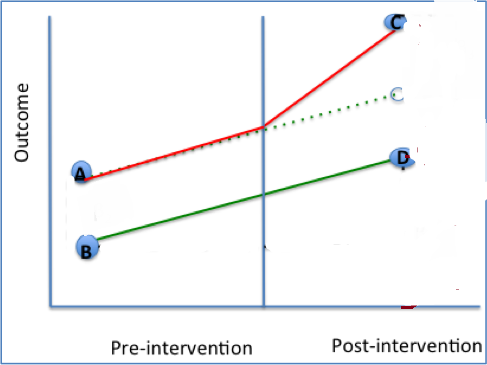
\includegraphics[width=0.7\textwidth,height=\textheight]{"images/DIDregressionblank.png"}
\caption{Green: Never Treated, Red: Treated}
\end{figure}
\end{frame}

\begin{frame}{The Parallel Trends Assumption:}
\protect\hypertarget{the-parallel-trends-assumption}{}
\begin{itemize}
\item
  We are treating the dashed green line as the counterfactual for the
  treated group
\item
  Any deviation from this counterfactual is attributed to the treatment
  effect
\item
  This assumption is straightforward but fundamentally
  \textbf{untestable}, because we will never actually observe this
  counterfactual of what would have happened to the treated group had
  they not been treated.
\end{itemize}
\end{frame}

\begin{frame}{DID visually:}
\protect\hypertarget{did-visually}{}
\[
Y_{it}=\beta_0+\beta_1 Post_t+\beta_2 GetsTreat_i+\beta_3 Post_t\times GetsTreat_i+u_{it}
\] Which number corresponds to which coefficient? \(\Rightarrow\) Top
Hat

\begin{figure}
\centering
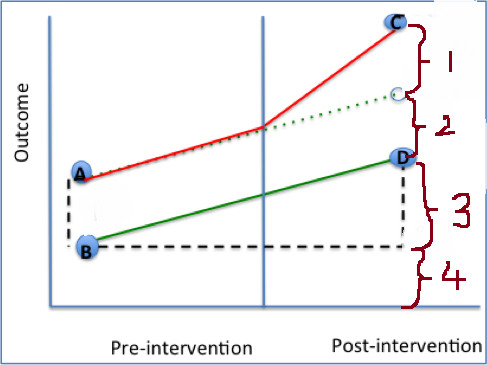
\includegraphics[width=0.7\textwidth,height=\textheight]{"images/DIDregression.png"}
\caption{Green: Never Treated, Red: Treated}
\end{figure}
\end{frame}

\begin{frame}{Identifying Assumption:}
\protect\hypertarget{identifying-assumption-1}{}
\[
Y_{it}=\beta_0+\beta_1 Post_t+\beta_2 GetsTreat_i+\beta_3 Post_t\times GetsTreat_i+u_{it}
\]

\begin{figure}
\centering
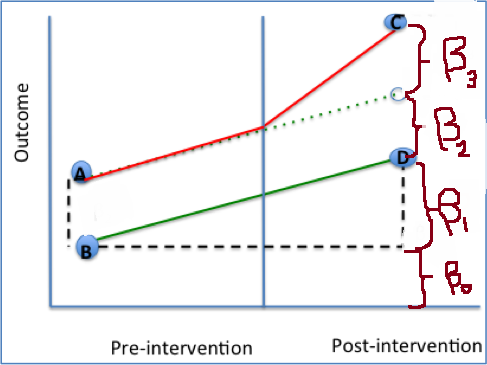
\includegraphics[width=0.7\textwidth,height=\textheight]{"images/DIDregressionnum.png"}
\caption{Green: Never Treated, Red: Treated}
\end{figure}
\end{frame}

\begin{frame}{Problems with the Parallel Trends assumption}
\protect\hypertarget{problems-with-the-parallel-trends-assumption}{}
The parallel trends assumption is a fairly big assumption in many
circumstances:

\begin{itemize}
\tightlist
\item
  policymakers may select treatment and control based on differences in
  the \textbf{anticipated} effects of treatment, or pre-existing
  differences in outcomes
\end{itemize}

In this case, the parallel trends assumption does not hold.
\end{frame}

\begin{frame}{Example: Ashenfelter dips}
\protect\hypertarget{example-ashenfelter-dips}{}
Individuals who are ``Treated'' by job training programs are often
individuals who just experienced a ``dip'' in earnings due to a job
loss. When they get rehired their earnings increase substantially.

\begin{itemize}
\item
  If I compare their change in earnings to the change experienced by
  people who did not sign up for job training, I will see a large
  differential increase in earnings associated with program
  participation.
\item
  This is due to who selects into training, not the causal effect of
  training.
\end{itemize}
\end{frame}

\begin{frame}{Verifying Parallel trends}
\protect\hypertarget{verifying-parallel-trends}{}
How can we check to see if the parallel trends assumption is likely to
hold?

\begin{itemize}
\item
  Fundamentally untestable assumption
\item
  use deduction to check this assumptions validity.
\end{itemize}

\(\Rightarrow\) if the pre-treatment trends were parallel between the
two groups, then wouldn't it stand to reason that the post-treatment
trends would have been too?

Note: parallel pre-treatment trends does not \textbf{\textit{prove}}
that the assumption holds. But it does give some confidence that it does
(absent some unobserved group specific time shock).
\end{frame}

\begin{frame}{Verifying Parallel trends}
\protect\hypertarget{verifying-parallel-trends-1}{}
Including leads into the DiD model is an easy way to check the
pre-treatment trends. (Lags can also be included to see if treatment
effect change over time).

Suppose treatment occurs right after period \(t=0\), estimate

\[
Y_{it}=\beta_0+\beta_2GetsTreat_i+\sum_{t=-n}^m\beta_{3t}Period_t \times GetsTreat_i+\lambda_t+u_{it}.
\]

If parallel trends holds:

\begin{itemize}
\item
  \(E[\hat{\beta}_{3,t<1}]=0\) since there is no treatment in these time
  periods.
\item
  If \(\tau\neq0\), \(E[\hat{\beta}_{3,t>0}]\neq0\).
\end{itemize}

These results are typically best presented graphically.
\end{frame}

\begin{frame}{Graphing DID estimates}
\protect\hypertarget{graphing-did-estimates}{}
Two main types of graphs

\begin{itemize}
\item
  plots of the mean outcome for both the treatment and control for
  several periods before and after treatment,
\item
  and/or a graph that plots the \(\hat{\beta}_{3t}\) estimates from the
  specification above.
\end{itemize}
\end{frame}

\begin{frame}[fragile]{Simulation: With leads and lags}
\protect\hypertarget{simulation-with-leads-and-lags}{}
\tiny

\begin{Shaded}
\begin{Highlighting}[]
\CommentTok{\# simulating the data}
\FunctionTok{set.seed}\NormalTok{(}\DecValTok{1999}\NormalTok{)}
\NormalTok{scoresbase }\OtherTok{\textless{}{-}} \FunctionTok{as.data.frame}\NormalTok{(}\FunctionTok{rep}\NormalTok{(}\FunctionTok{c}\NormalTok{(}\DecValTok{1}\NormalTok{, }\DecValTok{2}\NormalTok{, }\DecValTok{3}\NormalTok{, }\DecValTok{4}\NormalTok{, }\DecValTok{5}\NormalTok{, }\DecValTok{6}\NormalTok{, }\DecValTok{7}\NormalTok{, }\DecValTok{8}\NormalTok{, }\DecValTok{9}\NormalTok{,}
    \DecValTok{10}\NormalTok{), }\AttributeTok{times =} \DecValTok{30}\NormalTok{))}
\FunctionTok{names}\NormalTok{(scoresbase) }\OtherTok{\textless{}{-}} \FunctionTok{c}\NormalTok{(}\StringTok{"class"}\NormalTok{)}
\NormalTok{scoresbase }\OtherTok{\textless{}{-}}\NormalTok{ fastDummies}\SpecialCharTok{::}\FunctionTok{dummy\_cols}\NormalTok{(scoresbase, }\AttributeTok{select\_columns =} \StringTok{"class"}\NormalTok{)}

\CommentTok{\# suppose the better teachers (classes, 7,8,9,10) select to}
\CommentTok{\# participate in the book club program}
\NormalTok{scoresbase}\SpecialCharTok{$}\NormalTok{treat }\OtherTok{\textless{}{-}} \DecValTok{0}
\NormalTok{scoresbase}\SpecialCharTok{$}\NormalTok{treat[scoresbase}\SpecialCharTok{$}\NormalTok{class }\SpecialCharTok{\%in\%} \FunctionTok{c}\NormalTok{(}\DecValTok{7}\NormalTok{, }\DecValTok{8}\NormalTok{, }\DecValTok{9}\NormalTok{, }\DecValTok{10}\NormalTok{)] }\OtherTok{\textless{}{-}} \DecValTok{1}
\end{Highlighting}
\end{Shaded}
\end{frame}

\begin{frame}[fragile]{Simulation: With leads and lags}
\protect\hypertarget{simulation-with-leads-and-lags-1}{}
\tiny

\begin{Shaded}
\begin{Highlighting}[]
\CommentTok{\# Gnerating simulated data for each year using a for loop}
\NormalTok{yr }\OtherTok{\textless{}{-}} \FunctionTok{c}\NormalTok{(}\DecValTok{1995}\NormalTok{, }\DecValTok{1996}\NormalTok{, }\DecValTok{1997}\NormalTok{, }\DecValTok{1998}\NormalTok{, }\DecValTok{1999}\NormalTok{, }\DecValTok{2000}\NormalTok{, }\DecValTok{2001}\NormalTok{, }\DecValTok{2002}\NormalTok{, }\DecValTok{2003}\NormalTok{,}
    \DecValTok{2004}\NormalTok{, }\DecValTok{2005}\NormalTok{)}
\NormalTok{tauyr }\OtherTok{\textless{}{-}} \FunctionTok{c}\NormalTok{(}\DecValTok{0}\NormalTok{, }\DecValTok{0}\NormalTok{, }\DecValTok{0}\NormalTok{, }\DecValTok{0}\NormalTok{, }\DecValTok{0}\NormalTok{, }\DecValTok{0}\NormalTok{, }\DecValTok{10}\NormalTok{, }\DecValTok{10}\NormalTok{, }\DecValTok{10}\NormalTok{, }\DecValTok{10}\NormalTok{, }\DecValTok{10}\NormalTok{)}
\NormalTok{yrfe }\OtherTok{\textless{}{-}} \FunctionTok{c}\NormalTok{(}\DecValTok{72}\NormalTok{, }\DecValTok{77}\NormalTok{, }\DecValTok{75}\NormalTok{, }\DecValTok{79}\NormalTok{, }\DecValTok{81}\NormalTok{, }\DecValTok{79}\NormalTok{, }\DecValTok{83}\NormalTok{, }\DecValTok{77}\NormalTok{, }\DecValTok{82}\NormalTok{, }\DecValTok{84}\NormalTok{, }\DecValTok{81}\NormalTok{)}

\CommentTok{\# loop to generate the data}
\ControlFlowTok{for}\NormalTok{ (i }\ControlFlowTok{in} \DecValTok{1}\SpecialCharTok{:}\DecValTok{11}\NormalTok{) \{}
\NormalTok{    name }\OtherTok{\textless{}{-}} \FunctionTok{paste}\NormalTok{(}\StringTok{"scores"}\NormalTok{, yr[i], }\AttributeTok{sep =} \StringTok{"\_"}\NormalTok{)}
\NormalTok{    scores }\OtherTok{\textless{}{-}}\NormalTok{ scoresbase}
\NormalTok{    scores}\SpecialCharTok{$}\NormalTok{error }\OtherTok{\textless{}{-}} \FunctionTok{rnorm}\NormalTok{(}\DecValTok{300}\NormalTok{, }\AttributeTok{mean =} \DecValTok{0}\NormalTok{, }\AttributeTok{sd =} \DecValTok{10}\NormalTok{)}
\NormalTok{    tau }\OtherTok{\textless{}{-}}\NormalTok{ tauyr[i]}
\NormalTok{    yearfe }\OtherTok{\textless{}{-}}\NormalTok{ yrfe[i]}
    \CommentTok{\# the data generating process}
\NormalTok{    scores}\SpecialCharTok{$}\NormalTok{read4 }\OtherTok{\textless{}{-}}\NormalTok{ (yearfe }\SpecialCharTok{+}\NormalTok{ tau }\SpecialCharTok{*}\NormalTok{ scores}\SpecialCharTok{$}\NormalTok{treat }\SpecialCharTok{+}\NormalTok{ scores}\SpecialCharTok{$}\NormalTok{error }\SpecialCharTok{+}
\NormalTok{        (}\SpecialCharTok{{-}}\DecValTok{10}\NormalTok{) }\SpecialCharTok{*}\NormalTok{ scores}\SpecialCharTok{$}\NormalTok{class\_1 }\SpecialCharTok{+}\NormalTok{ (}\SpecialCharTok{{-}}\DecValTok{15}\NormalTok{) }\SpecialCharTok{*}\NormalTok{ scores}\SpecialCharTok{$}\NormalTok{class\_2 }\SpecialCharTok{+}\NormalTok{ (}\SpecialCharTok{{-}}\DecValTok{5}\NormalTok{) }\SpecialCharTok{*}
\NormalTok{        scores}\SpecialCharTok{$}\NormalTok{class\_3 }\SpecialCharTok{+}\NormalTok{ (}\SpecialCharTok{{-}}\DecValTok{8}\NormalTok{) }\SpecialCharTok{*}\NormalTok{ scores}\SpecialCharTok{$}\NormalTok{class\_4 }\SpecialCharTok{+}\NormalTok{ (}\SpecialCharTok{{-}}\DecValTok{7}\NormalTok{) }\SpecialCharTok{*}\NormalTok{ scores}\SpecialCharTok{$}\NormalTok{class\_5 }\SpecialCharTok{+}
\NormalTok{        (}\SpecialCharTok{{-}}\DecValTok{13}\NormalTok{) }\SpecialCharTok{*}\NormalTok{ scores}\SpecialCharTok{$}\NormalTok{class\_6 }\SpecialCharTok{+}\NormalTok{ (}\DecValTok{11}\NormalTok{) }\SpecialCharTok{*}\NormalTok{ scores}\SpecialCharTok{$}\NormalTok{class\_7 }\SpecialCharTok{+}\NormalTok{ (}\DecValTok{8}\NormalTok{) }\SpecialCharTok{*}
\NormalTok{        scores}\SpecialCharTok{$}\NormalTok{class\_8 }\SpecialCharTok{+}\NormalTok{ (}\DecValTok{10}\NormalTok{) }\SpecialCharTok{*}\NormalTok{ scores}\SpecialCharTok{$}\NormalTok{class\_9 }\SpecialCharTok{+}\NormalTok{ (}\DecValTok{12}\NormalTok{) }\SpecialCharTok{*}\NormalTok{ scores}\SpecialCharTok{$}\NormalTok{class\_10)}

\NormalTok{    scores}\SpecialCharTok{$}\NormalTok{year }\OtherTok{\textless{}{-}}\NormalTok{ yr[i]}
    \FunctionTok{assign}\NormalTok{(name, scores)}
    \FunctionTok{rm}\NormalTok{(scores)}
\NormalTok{\}}

\NormalTok{allscores }\OtherTok{\textless{}{-}} \FunctionTok{rbind}\NormalTok{(scores\_1995, scores\_1996, scores\_1997, scores\_1998,}
\NormalTok{    scores\_1999, scores\_2000, scores\_2001, scores\_2002, scores\_2003,}
\NormalTok{    scores\_2004, scores\_2005)}
\end{Highlighting}
\end{Shaded}
\end{frame}

\begin{frame}[fragile]{Simulation: With leads and lags}
\protect\hypertarget{simulation-with-leads-and-lags-2}{}
\tiny

\begin{Shaded}
\begin{Highlighting}[]
\NormalTok{allscores}\SpecialCharTok{$}\NormalTok{post }\OtherTok{\textless{}{-}} \DecValTok{0}
\NormalTok{allscores}\SpecialCharTok{$}\NormalTok{post[allscores}\SpecialCharTok{$}\NormalTok{year }\SpecialCharTok{\%in\%} \FunctionTok{c}\NormalTok{(}\DecValTok{2001}\NormalTok{, }\DecValTok{2002}\NormalTok{, }\DecValTok{2003}\NormalTok{, }\DecValTok{2004}\NormalTok{,}
    \DecValTok{2005}\NormalTok{)] }\OtherTok{\textless{}{-}} \DecValTok{1}

\NormalTok{allscores }\OtherTok{\textless{}{-}}\NormalTok{ fastDummies}\SpecialCharTok{::}\FunctionTok{dummy\_cols}\NormalTok{(allscores, }\AttributeTok{select\_columns =} \StringTok{"year"}\NormalTok{)}

\NormalTok{regdidall2 }\OtherTok{\textless{}{-}} \FunctionTok{felm}\NormalTok{(read4 }\SpecialCharTok{\textasciitilde{}}\NormalTok{ treat }\SpecialCharTok{+}\NormalTok{ year\_1995 }\SpecialCharTok{+}\NormalTok{ year\_1996 }\SpecialCharTok{+}\NormalTok{ year\_1997 }\SpecialCharTok{+}
\NormalTok{    year\_1998 }\SpecialCharTok{+}\NormalTok{ year\_1999 }\SpecialCharTok{+}\NormalTok{ year\_2001 }\SpecialCharTok{+}\NormalTok{ year\_2002 }\SpecialCharTok{+}\NormalTok{ year\_2003 }\SpecialCharTok{+}
\NormalTok{    year\_2004 }\SpecialCharTok{+}\NormalTok{ year\_2005 }\SpecialCharTok{+}\NormalTok{ year\_1995 }\SpecialCharTok{*}\NormalTok{ treat }\SpecialCharTok{+}\NormalTok{ year\_1996 }\SpecialCharTok{*}\NormalTok{ treat }\SpecialCharTok{+}
\NormalTok{    year\_1997 }\SpecialCharTok{*}\NormalTok{ treat }\SpecialCharTok{+}\NormalTok{ year\_1998 }\SpecialCharTok{*}\NormalTok{ treat }\SpecialCharTok{+}\NormalTok{ year\_1999 }\SpecialCharTok{*}\NormalTok{ treat }\SpecialCharTok{+}
\NormalTok{    year\_2001 }\SpecialCharTok{*}\NormalTok{ treat }\SpecialCharTok{+}\NormalTok{ year\_2002 }\SpecialCharTok{*}\NormalTok{ treat }\SpecialCharTok{+}\NormalTok{ year\_2003 }\SpecialCharTok{*}\NormalTok{ treat }\SpecialCharTok{+}
\NormalTok{    year\_2004 }\SpecialCharTok{*}\NormalTok{ treat }\SpecialCharTok{+}\NormalTok{ year\_2005 }\SpecialCharTok{*}\NormalTok{ treat, allscores)}
\end{Highlighting}
\end{Shaded}
\end{frame}

\begin{frame}[fragile]{Simulation: With leads and lags}
\protect\hypertarget{simulation-with-leads-and-lags-3}{}
\tiny

\begin{Shaded}
\begin{Highlighting}[]
\FunctionTok{stargazer}\NormalTok{(regdidall2, }\AttributeTok{type =} \StringTok{"latex"}\NormalTok{, }\AttributeTok{no.space =} \ConstantTok{TRUE}\NormalTok{, }\AttributeTok{header =} \ConstantTok{FALSE}\NormalTok{,}
    \AttributeTok{single.row =} \ConstantTok{TRUE}\NormalTok{, }\AttributeTok{omit.stat =} \StringTok{"all"}\NormalTok{)}
\end{Highlighting}
\end{Shaded}

\begin{table}[!htbp] \centering 
  \caption{} 
  \label{} 
\begin{tabular}{@{\extracolsep{5pt}}lc} 
\\[-1.8ex]\hline 
\hline \\[-1.8ex] 
 & \multicolumn{1}{c}{\textit{Dependent variable:}} \\ 
\cline{2-2} 
\\[-1.8ex] & read4 \\ 
\hline \\[-1.8ex] 
 treat & 18.774$^{***}$ (1.207) \\ 
  year\_1995 & $-$5.842$^{***}$ (1.080) \\ 
  year\_1996 & $-$2.945$^{***}$ (1.080) \\ 
  year\_1997 & $-$1.696 (1.080) \\ 
  year\_1998 & 0.027 (1.080) \\ 
  year\_1999 & 2.636$^{**}$ (1.080) \\ 
  year\_2001 & 5.125$^{***}$ (1.080) \\ 
  year\_2002 & $-$2.235$^{**}$ (1.080) \\ 
  year\_2003 & 1.849$^{*}$ (1.080) \\ 
  year\_2004 & 4.430$^{***}$ (1.080) \\ 
  year\_2005 & 2.533$^{**}$ (1.080) \\ 
  treat:year\_1995 & 0.431 (1.707) \\ 
  treat:year\_1996 & 1.427 (1.707) \\ 
  treat:year\_1997 & $-$2.476 (1.707) \\ 
  treat:year\_1998 & 0.568 (1.707) \\ 
  treat:year\_1999 & $-$0.573 (1.707) \\ 
  treat:year\_2001 & 10.204$^{***}$ (1.707) \\ 
  treat:year\_2002 & 12.290$^{***}$ (1.707) \\ 
  treat:year\_2003 & 11.188$^{***}$ (1.707) \\ 
  treat:year\_2004 & 11.186$^{***}$ (1.707) \\ 
  treat:year\_2005 & 10.217$^{***}$ (1.707) \\ 
  Constant & 69.542$^{***}$ (0.764) \\ 
 \hline \\[-1.8ex] 
\hline 
\hline \\[-1.8ex] 
\textit{Note:}  & \multicolumn{1}{r}{$^{*}$p$<$0.1; $^{**}$p$<$0.05; $^{***}$p$<$0.01} \\ 
\end{tabular} 
\end{table}
\end{frame}

\begin{frame}[fragile]{Simulation: With leads and lags}
\protect\hypertarget{simulation-with-leads-and-lags-4}{}
\tiny

\begin{Shaded}
\begin{Highlighting}[]
\CommentTok{\# start with plot of group means}

\CommentTok{\# calculateing the mean score for each year by treatment}
\CommentTok{\# status}
\NormalTok{grp\_mean }\OtherTok{\textless{}{-}}\NormalTok{ allscores }\SpecialCharTok{\%\textgreater{}\%}
    \FunctionTok{group\_by}\NormalTok{(year, treat) }\SpecialCharTok{\%\textgreater{}\%}
\NormalTok{    dplyr}\SpecialCharTok{::}\FunctionTok{summarize}\NormalTok{(}\AttributeTok{groupmean =} \FunctionTok{mean}\NormalTok{(read4, }\AttributeTok{na.rm =} \ConstantTok{TRUE}\NormalTok{))}
\end{Highlighting}
\end{Shaded}

\begin{verbatim}
## `summarise()` has grouped output by 'year'. You can override using the
## `.groups` argument.
\end{verbatim}

\begin{Shaded}
\begin{Highlighting}[]
\NormalTok{grp\_mean}\SpecialCharTok{$}\NormalTok{treat }\OtherTok{\textless{}{-}} \FunctionTok{as.factor}\NormalTok{(grp\_mean}\SpecialCharTok{$}\NormalTok{treat)}

\CommentTok{\# difference in means plot}
\NormalTok{didmeans }\OtherTok{\textless{}{-}} \FunctionTok{ggplot}\NormalTok{(grp\_mean, }\FunctionTok{aes}\NormalTok{(year, groupmean, }\AttributeTok{group =}\NormalTok{ treat,}
    \AttributeTok{color =}\NormalTok{ treat)) }\SpecialCharTok{+} \FunctionTok{stat\_summary}\NormalTok{(}\AttributeTok{geom =} \StringTok{"line"}\NormalTok{) }\SpecialCharTok{+} \FunctionTok{geom\_vline}\NormalTok{(}\AttributeTok{xintercept =} \DecValTok{2000}\NormalTok{) }\SpecialCharTok{+}
    \FunctionTok{theme\_minimal}\NormalTok{()}
\end{Highlighting}
\end{Shaded}
\end{frame}

\begin{frame}{Simulation: With leads and lags}
\protect\hypertarget{simulation-with-leads-and-lags-5}{}
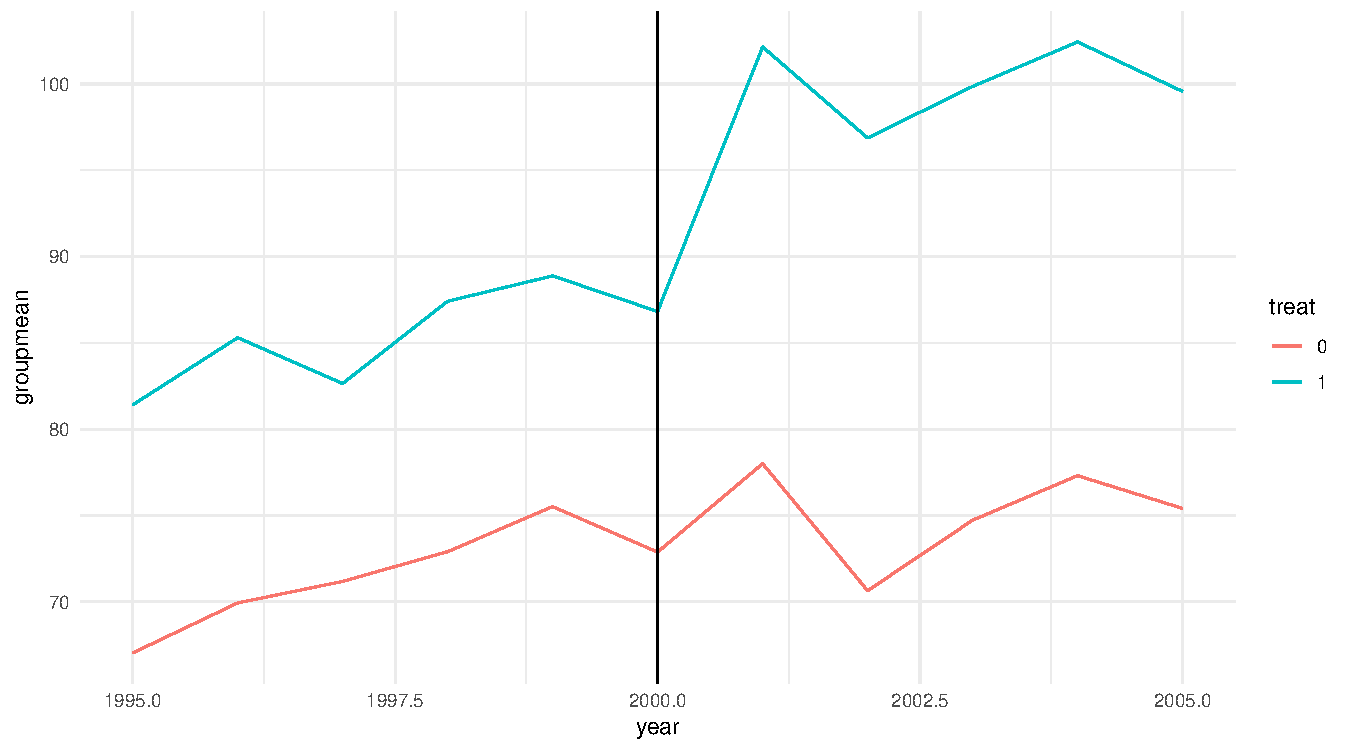
\includegraphics{"Slides_DID_files/figure-beamer/didplot-1.pdf"}
\end{frame}

\begin{frame}[fragile]{Simulation: With leads and lags}
\protect\hypertarget{simulation-with-leads-and-lags-6}{}
\tiny

\begin{Shaded}
\begin{Highlighting}[]
\CommentTok{\# plot of differences coefficients}

\NormalTok{res }\OtherTok{\textless{}{-}} \FunctionTok{coef}\NormalTok{(}\FunctionTok{summary}\NormalTok{(regdidall2))}
\NormalTok{res }\OtherTok{\textless{}{-}} \FunctionTok{as.data.frame}\NormalTok{(res)}

\NormalTok{res }\OtherTok{\textless{}{-}}\NormalTok{ res[}\DecValTok{13}\SpecialCharTok{:}\DecValTok{22}\NormalTok{, ]}

\NormalTok{a }\OtherTok{\textless{}{-}} \FunctionTok{c}\NormalTok{(}\DecValTok{0}\NormalTok{, }\DecValTok{0}\NormalTok{, }\DecValTok{0}\NormalTok{, }\DecValTok{0}\NormalTok{)}

\NormalTok{res }\OtherTok{\textless{}{-}} \FunctionTok{rbind}\NormalTok{(res, a)}

\NormalTok{year }\OtherTok{\textless{}{-}} \FunctionTok{c}\NormalTok{(}\DecValTok{1995}\NormalTok{, }\DecValTok{1996}\NormalTok{, }\DecValTok{1997}\NormalTok{, }\DecValTok{1998}\NormalTok{, }\DecValTok{1999}\NormalTok{, }\DecValTok{2001}\NormalTok{, }\DecValTok{2002}\NormalTok{, }\DecValTok{2003}\NormalTok{, }\DecValTok{2004}\NormalTok{,}
    \DecValTok{2005}\NormalTok{, }\DecValTok{2000}\NormalTok{)}
\NormalTok{res }\OtherTok{\textless{}{-}} \FunctionTok{cbind}\NormalTok{(res, year)}
\NormalTok{res}\SpecialCharTok{$}\NormalTok{ci }\OtherTok{\textless{}{-}} \FloatTok{1.96} \SpecialCharTok{*}\NormalTok{ res}\SpecialCharTok{$}\StringTok{\textasciigrave{}}\AttributeTok{Std. Error}\StringTok{\textasciigrave{}}

\FunctionTok{names}\NormalTok{(res) }\OtherTok{\textless{}{-}} \FunctionTok{c}\NormalTok{(}\StringTok{"Estimate"}\NormalTok{, }\StringTok{"se"}\NormalTok{, }\StringTok{"t"}\NormalTok{, }\StringTok{"p"}\NormalTok{, }\StringTok{"year"}\NormalTok{, }\StringTok{"ci"}\NormalTok{)}
\CommentTok{\# Use 95\% confidence interval instead of SEM}
\NormalTok{didplot2 }\OtherTok{\textless{}{-}} \FunctionTok{ggplot}\NormalTok{(res, }\FunctionTok{aes}\NormalTok{(}\AttributeTok{x =}\NormalTok{ year, }\AttributeTok{y =}\NormalTok{ Estimate)) }\SpecialCharTok{+} \FunctionTok{geom\_errorbar}\NormalTok{(}\FunctionTok{aes}\NormalTok{(}\AttributeTok{ymin =}\NormalTok{ Estimate }\SpecialCharTok{{-}}
\NormalTok{    ci, }\AttributeTok{ymax =}\NormalTok{ Estimate }\SpecialCharTok{+}\NormalTok{ ci), }\AttributeTok{width =} \FloatTok{0.1}\NormalTok{) }\SpecialCharTok{+} \FunctionTok{geom\_vline}\NormalTok{(}\AttributeTok{xintercept =} \DecValTok{2000}\NormalTok{) }\SpecialCharTok{+}
    \FunctionTok{geom\_hline}\NormalTok{(}\AttributeTok{yintercept =} \DecValTok{0}\NormalTok{) }\SpecialCharTok{+} \FunctionTok{geom\_point}\NormalTok{()}
\end{Highlighting}
\end{Shaded}
\end{frame}

\begin{frame}{Simulation: With leads and Lags}
\protect\hypertarget{simulation-with-leads-and-lags-7}{}
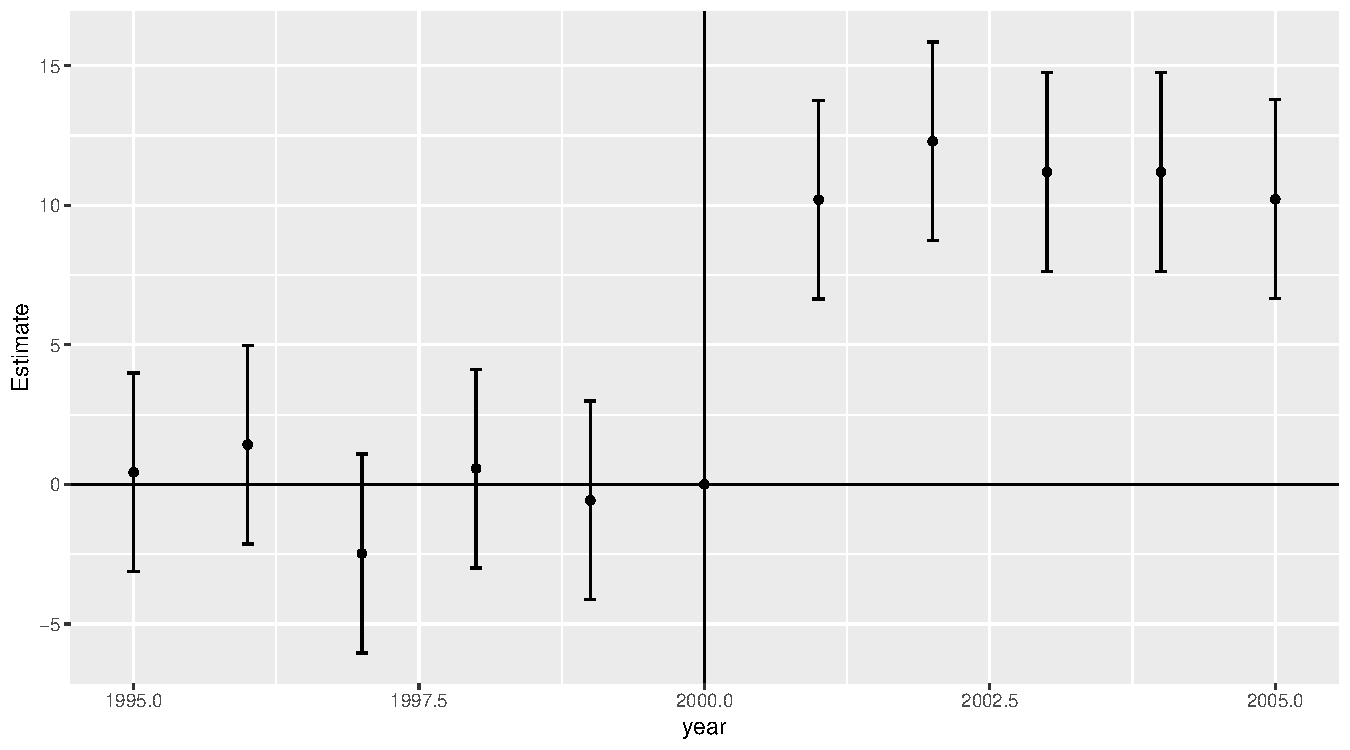
\includegraphics{"Slides_DID_files/figure-beamer/didplotb-1.pdf"}
\end{frame}

\begin{frame}{A note on Inference: Clustering}
\protect\hypertarget{a-note-on-inference-clustering}{}
What if the variable of interest only varies at a ``group'' level

\begin{itemize}
\item
  ex: at the state or class level
\item
  \(\Rightarrow\) observations are related with each other within
  certain groups
\item
  There is less variation then we actually think
\end{itemize}

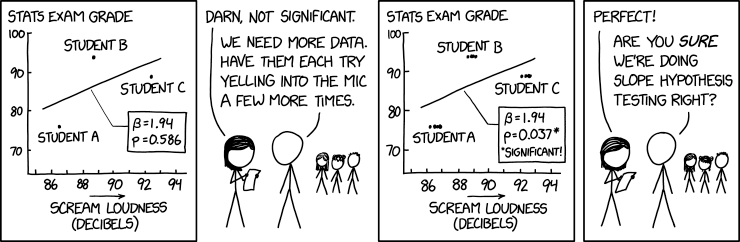
\includegraphics[width=0.9\textwidth,height=\textheight]{"images/cluster_comic.png"}
\end{frame}

\begin{frame}[fragile]{A note on Inference: Clustering}
\protect\hypertarget{a-note-on-inference-clustering-1}{}
Conventional standard errors will often severely understate the standard
deviation of the estimators and lead to inference errors.

Solution: cluster standard errors at the group level.

Clustering standard errors can be done in R using the felm function:
\tiny

\begin{Shaded}
\begin{Highlighting}[]
\NormalTok{regdidall3 }\OtherTok{\textless{}{-}} \FunctionTok{felm}\NormalTok{(read4 }\SpecialCharTok{\textasciitilde{}}\NormalTok{ treat }\SpecialCharTok{+}\NormalTok{ year\_1995 }\SpecialCharTok{+}\NormalTok{ year\_1996 }\SpecialCharTok{+}\NormalTok{ year\_1997 }\SpecialCharTok{+}
\NormalTok{    year\_1998 }\SpecialCharTok{+}\NormalTok{ year\_1999 }\SpecialCharTok{+}\NormalTok{ year\_2001 }\SpecialCharTok{+}\NormalTok{ year\_2002 }\SpecialCharTok{+}\NormalTok{ year\_2003 }\SpecialCharTok{+}
\NormalTok{    year\_2004 }\SpecialCharTok{+}\NormalTok{ year\_2005 }\SpecialCharTok{+}\NormalTok{ year\_1995 }\SpecialCharTok{*}\NormalTok{ treat }\SpecialCharTok{+}\NormalTok{ year\_1996 }\SpecialCharTok{*}\NormalTok{ treat }\SpecialCharTok{+}
\NormalTok{    year\_1997 }\SpecialCharTok{*}\NormalTok{ treat }\SpecialCharTok{+}\NormalTok{ year\_1998 }\SpecialCharTok{*}\NormalTok{ treat }\SpecialCharTok{+}\NormalTok{ year\_1999 }\SpecialCharTok{*}\NormalTok{ treat }\SpecialCharTok{+}
\NormalTok{    year\_2001 }\SpecialCharTok{*}\NormalTok{ treat }\SpecialCharTok{+}\NormalTok{ year\_2002 }\SpecialCharTok{*}\NormalTok{ treat }\SpecialCharTok{+}\NormalTok{ year\_2003 }\SpecialCharTok{*}\NormalTok{ treat }\SpecialCharTok{+}
\NormalTok{    year\_2004 }\SpecialCharTok{*}\NormalTok{ treat }\SpecialCharTok{+}\NormalTok{ year\_2005 }\SpecialCharTok{*}\NormalTok{ treat }\SpecialCharTok{|} \DecValTok{0} \SpecialCharTok{|} \DecValTok{0} \SpecialCharTok{|}\NormalTok{ class, allscores)}
\end{Highlighting}
\end{Shaded}
\end{frame}

\begin{frame}[fragile]{A note on Inference: Clustering}
\protect\hypertarget{a-note-on-inference-clustering-2}{}
\tiny

\begin{Shaded}
\begin{Highlighting}[]
\FunctionTok{stargazer}\NormalTok{(regdidall2, regdidall3, }\AttributeTok{type =} \StringTok{"latex"}\NormalTok{, }\AttributeTok{no.space =} \ConstantTok{TRUE}\NormalTok{,}
    \AttributeTok{single.row =} \ConstantTok{TRUE}\NormalTok{, }\AttributeTok{omit.stat =} \StringTok{"all"}\NormalTok{, }\AttributeTok{header =} \ConstantTok{FALSE}\NormalTok{)}
\end{Highlighting}
\end{Shaded}

\begin{table}[!htbp] \centering 
  \caption{} 
  \label{} 
\begin{tabular}{@{\extracolsep{5pt}}lcc} 
\\[-1.8ex]\hline 
\hline \\[-1.8ex] 
 & \multicolumn{2}{c}{\textit{Dependent variable:}} \\ 
\cline{2-3} 
\\[-1.8ex] & \multicolumn{2}{c}{read4} \\ 
\\[-1.8ex] & (1) & (2)\\ 
\hline \\[-1.8ex] 
 treat & 18.774$^{***}$ (1.207) & 18.774$^{***}$ (2.268) \\ 
  year\_1995 & $-$5.842$^{***}$ (1.080) & $-$5.842$^{***}$ (0.879) \\ 
  year\_1996 & $-$2.945$^{***}$ (1.080) & $-$2.945$^{***}$ (1.070) \\ 
  year\_1997 & $-$1.696 (1.080) & $-$1.696 (1.032) \\ 
  year\_1998 & 0.027 (1.080) & 0.027 (0.257) \\ 
  year\_1999 & 2.636$^{**}$ (1.080) & 2.636$^{**}$ (1.237) \\ 
  year\_2001 & 5.125$^{***}$ (1.080) & 5.125$^{***}$ (0.941) \\ 
  year\_2002 & $-$2.235$^{**}$ (1.080) & $-$2.235 (1.582) \\ 
  year\_2003 & 1.849$^{*}$ (1.080) & 1.849$^{***}$ (0.654) \\ 
  year\_2004 & 4.430$^{***}$ (1.080) & 4.430$^{***}$ (1.206) \\ 
  year\_2005 & 2.533$^{**}$ (1.080) & 2.533$^{***}$ (0.746) \\ 
  treat:year\_1995 & 0.431 (1.707) & 0.431 (1.768) \\ 
  treat:year\_1996 & 1.427 (1.707) & 1.427 (2.108) \\ 
  treat:year\_1997 & $-$2.476 (1.707) & $-$2.476$^{*}$ (1.287) \\ 
  treat:year\_1998 & 0.568 (1.707) & 0.568 (1.570) \\ 
  treat:year\_1999 & $-$0.573 (1.707) & $-$0.573 (1.477) \\ 
  treat:year\_2001 & 10.204$^{***}$ (1.707) & 10.204$^{***}$ (1.602) \\ 
  treat:year\_2002 & 12.290$^{***}$ (1.707) & 12.290$^{***}$ (2.310) \\ 
  treat:year\_2003 & 11.188$^{***}$ (1.707) & 11.188$^{***}$ (1.824) \\ 
  treat:year\_2004 & 11.186$^{***}$ (1.707) & 11.186$^{***}$ (2.216) \\ 
  treat:year\_2005 & 10.217$^{***}$ (1.707) & 10.217$^{***}$ (1.510) \\ 
  Constant & 69.542$^{***}$ (0.764) & 69.542$^{***}$ (1.965) \\ 
 \hline \\[-1.8ex] 
\hline 
\hline \\[-1.8ex] 
\textit{Note:}  & \multicolumn{2}{r}{$^{*}$p$<$0.1; $^{**}$p$<$0.05; $^{***}$p$<$0.01} \\ 
\end{tabular} 
\end{table}
\end{frame}

\begin{frame}{Falsification Tests: Alternative outcomes}
\protect\hypertarget{falsification-tests-alternative-outcomes}{}
In addition to checking for parallel pre-trends, you can also check and
see if there is a pattern of parallel trends for an alternative outcome
measure that should not be affected by treatment.

For the ERS example,

\begin{itemize}
\item
  estimate the same model with manslaughter or male murders as the
  outcome variable.
\item
  these variables would be affected by the underlying violent crime in
  the city, but should be unaffected by ERS.
\end{itemize}
\end{frame}

\begin{frame}{Falsification Tests: Triple differences}
\protect\hypertarget{falsification-tests-triple-differences}{}
Adding another layer of differencing to the estimator (a triple-diff
estimator) can make DID results more compelling.

In our simulated example:

\begin{itemize}
\item
  Suppose a subset of students already had access to the book club
  through an after school program.
\item
  We can use the students in the after school program as an additional
  ``control'' group, since their performance should not change when the
  book club is introduced to the classrooms.
\end{itemize}
\end{frame}

\begin{frame}{Falsification Tests: Triple differences}
\protect\hypertarget{falsification-tests-triple-differences-1}{}
Let \(\bar{Y}_{a,g,t}\) represent the mean reading score of students

\begin{itemize}
\item
  in group \(g\) (control or treatment classes)
\item
  in year \(t\)
\item
  that are (\(a=AS\)) or are not (\(a=NAS\)) in the after school
  program.
\end{itemize}

The triple difference estimator is then \footnotesize \[
[(\bar{Y}_{T,1,AS}-\bar{Y}_{T,1,NAS})-(\bar{Y}_{T,0,AS}-\bar{Y}_{T,0,NAS})]-[(\bar{Y}_{C,1, AS}-\bar{Y}_{C,1, NAS})-(\bar{Y}_{C,0,AS}-\bar{Y}_{C,0,NAS})]
\] \normalsize \(\Rightarrow\) we compare the evolution of the gap
between the after school kids and the others in the treated classrooms
to the evolution of the gap between after school kids and the others in
the control classrooms.
\end{frame}

\begin{frame}{Falsification Tests: Triple differences}
\protect\hypertarget{falsification-tests-triple-differences-2}{}
Triple difference estimation allows us to relax some assumptions:

\begin{itemize}
\item
  We no longer need to assume that outcomes for treated and control
  would evolve similarly in expectation-
\item
  we now only need to assume that, to the extent that outcomes evolve
  differently in treated and control classes, the difference affects
  participants and non-participants in the after school program
  similarly.
\end{itemize}
\end{frame}

\begin{frame}{Triple differences}
\protect\hypertarget{triple-differences}{}
Triple diff regressions: Lots of interation terms!

\begin{itemize}
\item
  Put in an indicator for every main effect and interaction up to, but
  not including, the level at which the treatment varies.
\item
  We include the main effects for time, class and after-school program
  participation as well as all possible two way interactions between
  each of these indicators.
\end{itemize}

The regression looks like this:

\[
\begin{aligned}
Y_{i,a,g,t}=&\alpha_0+\alpha_1 GetT_{g}+\alpha_2 AS_{a}+\alpha_3 Post_{t}\\
&+\alpha_4 (GetT \times Post)_{gt}+\alpha_5 (GetT \times AS)_{ga}+\alpha_6 (Post \times AS)_{ta}\\
&+\alpha_7 (GetT \times Post \times AS)_{agt}+u_{igta}
\end{aligned}
\]
\end{frame}

\begin{frame}{Triple differences}
\protect\hypertarget{triple-differences-1}{}
\[
\begin{aligned}
Y_{i,a,g,t}=&\alpha_0+\alpha_1 GetT_{g}+\alpha_2 AS_{a}+\alpha_3 Post_{t}\\
&+\alpha_4 (GetT \times Post)_{gt}+\alpha_5 (GetT \times AS)_{ga}+\alpha_6 (Post \times AS)_{ta}\\
&+\alpha_7 (GetT \times Post \times AS)_{agt}+u_{igta}
\end{aligned}
\] What is the alternative hypothesis, stated in terms of these
coefficients?

\(\Rightarrow\) Top Hat
\end{frame}

\begin{frame}{Triple differences}
\protect\hypertarget{triple-differences-2}{}
Where will we see the treatment effect?

\begin{itemize}
\item
  Students who are not in the after school program (\(AS=0\))
\item
  When the the treated classes (\(GetT=1\)) adopt the book club
\item
  When treatment is implemented\(Post=1\),
\end{itemize}

\(\Rightarrow\) we would expect the treatment effect to manifest as:

\begin{itemize}
\item
  \(\alpha_4>0\)
\item
  \(\alpha_4+\alpha_7=0\) (since the after school kids experience no
  change in the post period).
\end{itemize}
\end{frame}

\begin{frame}[fragile]{Triple differences: Simulation}
\protect\hypertarget{triple-differences-simulation}{}
I simulate a new set of reading scores that based on a DGP that includes
the after school program effects.

\tiny

\begin{Shaded}
\begin{Highlighting}[]
\FunctionTok{set.seed}\NormalTok{(}\DecValTok{123456}\NormalTok{)}
\NormalTok{scores }\OtherTok{\textless{}{-}} \FunctionTok{as.data.frame}\NormalTok{(}\FunctionTok{rep}\NormalTok{(}\FunctionTok{c}\NormalTok{(}\DecValTok{1}\NormalTok{, }\DecValTok{2}\NormalTok{, }\DecValTok{3}\NormalTok{, }\DecValTok{4}\NormalTok{, }\DecValTok{5}\NormalTok{, }\DecValTok{6}\NormalTok{, }\DecValTok{7}\NormalTok{, }\DecValTok{8}\NormalTok{, }\DecValTok{9}\NormalTok{, }\DecValTok{10}\NormalTok{),}
    \AttributeTok{times =} \DecValTok{30}\NormalTok{))}
\FunctionTok{names}\NormalTok{(scores) }\OtherTok{\textless{}{-}} \FunctionTok{c}\NormalTok{(}\StringTok{"class"}\NormalTok{)}
\NormalTok{scores }\OtherTok{\textless{}{-}}\NormalTok{ fastDummies}\SpecialCharTok{::}\FunctionTok{dummy\_cols}\NormalTok{(scores, }\AttributeTok{select\_columns =} \StringTok{"class"}\NormalTok{)}

\NormalTok{scores}\SpecialCharTok{$}\NormalTok{error }\OtherTok{\textless{}{-}} \FunctionTok{rnorm}\NormalTok{(}\DecValTok{300}\NormalTok{, }\AttributeTok{mean =} \DecValTok{0}\NormalTok{, }\AttributeTok{sd =} \DecValTok{10}\NormalTok{)}

\CommentTok{\# a random indicator for participation in the afterschool}
\CommentTok{\# program}
\NormalTok{scores}\SpecialCharTok{$}\NormalTok{aftsch }\OtherTok{\textless{}{-}} \FunctionTok{rbinom}\NormalTok{(}\DecValTok{300}\NormalTok{, }\DecValTok{1}\NormalTok{, }\FloatTok{0.5}\NormalTok{)}

\CommentTok{\# suppose the best teachers (classes, 7,8,9,10) select into}
\CommentTok{\# participating in the book club program}
\NormalTok{scores}\SpecialCharTok{$}\NormalTok{treat }\OtherTok{\textless{}{-}} \DecValTok{0}
\NormalTok{scores}\SpecialCharTok{$}\NormalTok{treat[scores}\SpecialCharTok{$}\NormalTok{class }\SpecialCharTok{\%in\%} \FunctionTok{c}\NormalTok{(}\DecValTok{7}\NormalTok{, }\DecValTok{8}\NormalTok{, }\DecValTok{9}\NormalTok{, }\DecValTok{10}\NormalTok{)] }\OtherTok{\textless{}{-}} \DecValTok{1}

\CommentTok{\# creating an indicator for students who are become treated}
\CommentTok{\# and are not in the after school program}
\NormalTok{scores}\SpecialCharTok{$}\NormalTok{treatnotaftsch }\OtherTok{\textless{}{-}} \DecValTok{0}
\NormalTok{scores}\SpecialCharTok{$}\NormalTok{treatnotaftsch[scores}\SpecialCharTok{$}\NormalTok{treat }\SpecialCharTok{==} \DecValTok{1} \SpecialCharTok{\&}\NormalTok{ scores}\SpecialCharTok{$}\NormalTok{aftsch }\SpecialCharTok{==} \DecValTok{0}\NormalTok{] }\OtherTok{\textless{}{-}} \DecValTok{1}

\CommentTok{\# the treatment effect}
\NormalTok{tau }\OtherTok{\textless{}{-}} \DecValTok{10}

\CommentTok{\# the data generating process}
\NormalTok{scores}\SpecialCharTok{$}\NormalTok{read4 }\OtherTok{\textless{}{-}}\NormalTok{ (}\DecValTok{85} \SpecialCharTok{+} \DecValTok{13} \SpecialCharTok{*}\NormalTok{ scores}\SpecialCharTok{$}\NormalTok{aftsch }\SpecialCharTok{+}\NormalTok{ tau }\SpecialCharTok{*}\NormalTok{ scores}\SpecialCharTok{$}\NormalTok{treatnotaftsch }\SpecialCharTok{+}
\NormalTok{    scores}\SpecialCharTok{$}\NormalTok{error }\SpecialCharTok{+}\NormalTok{ (}\SpecialCharTok{{-}}\DecValTok{10}\NormalTok{) }\SpecialCharTok{*}\NormalTok{ scores}\SpecialCharTok{$}\NormalTok{class\_1 }\SpecialCharTok{+}\NormalTok{ (}\SpecialCharTok{{-}}\DecValTok{15}\NormalTok{) }\SpecialCharTok{*}\NormalTok{ scores}\SpecialCharTok{$}\NormalTok{class\_2 }\SpecialCharTok{+}
\NormalTok{    (}\SpecialCharTok{{-}}\DecValTok{5}\NormalTok{) }\SpecialCharTok{*}\NormalTok{ scores}\SpecialCharTok{$}\NormalTok{class\_3 }\SpecialCharTok{+}\NormalTok{ (}\SpecialCharTok{{-}}\DecValTok{8}\NormalTok{) }\SpecialCharTok{*}\NormalTok{ scores}\SpecialCharTok{$}\NormalTok{class\_4 }\SpecialCharTok{+}\NormalTok{ (}\SpecialCharTok{{-}}\DecValTok{3}\NormalTok{) }\SpecialCharTok{*}\NormalTok{ scores}\SpecialCharTok{$}\NormalTok{class\_5 }\SpecialCharTok{+}
\NormalTok{    (}\DecValTok{3}\NormalTok{) }\SpecialCharTok{*}\NormalTok{ scores}\SpecialCharTok{$}\NormalTok{class\_6 }\SpecialCharTok{+}\NormalTok{ (}\DecValTok{5}\NormalTok{) }\SpecialCharTok{*}\NormalTok{ scores}\SpecialCharTok{$}\NormalTok{class\_7 }\SpecialCharTok{+}\NormalTok{ (}\DecValTok{8}\NormalTok{) }\SpecialCharTok{*}\NormalTok{ scores}\SpecialCharTok{$}\NormalTok{class\_8 }\SpecialCharTok{+}
\NormalTok{    (}\DecValTok{10}\NormalTok{) }\SpecialCharTok{*}\NormalTok{ scores}\SpecialCharTok{$}\NormalTok{class\_9 }\SpecialCharTok{+}\NormalTok{ (}\DecValTok{12}\NormalTok{) }\SpecialCharTok{*}\NormalTok{ scores}\SpecialCharTok{$}\NormalTok{class\_10)}

\NormalTok{scores}\SpecialCharTok{$}\NormalTok{year }\OtherTok{\textless{}{-}} \StringTok{"2001"}

\NormalTok{scores01 }\OtherTok{\textless{}{-}}\NormalTok{ scores}
\FunctionTok{rm}\NormalTok{(scores)}
\end{Highlighting}
\end{Shaded}
\end{frame}

\begin{frame}[fragile]{Triple differences: Simulation}
\protect\hypertarget{triple-differences-simulation-1}{}
\tiny

\begin{Shaded}
\begin{Highlighting}[]
\NormalTok{scores }\OtherTok{\textless{}{-}} \FunctionTok{as.data.frame}\NormalTok{(}\FunctionTok{rep}\NormalTok{(}\FunctionTok{c}\NormalTok{(}\DecValTok{1}\NormalTok{, }\DecValTok{2}\NormalTok{, }\DecValTok{3}\NormalTok{, }\DecValTok{4}\NormalTok{, }\DecValTok{5}\NormalTok{, }\DecValTok{6}\NormalTok{, }\DecValTok{7}\NormalTok{, }\DecValTok{8}\NormalTok{, }\DecValTok{9}\NormalTok{, }\DecValTok{10}\NormalTok{),}
    \AttributeTok{times =} \DecValTok{30}\NormalTok{))}
\FunctionTok{names}\NormalTok{(scores) }\OtherTok{\textless{}{-}} \FunctionTok{c}\NormalTok{(}\StringTok{"class"}\NormalTok{)}
\NormalTok{scores }\OtherTok{\textless{}{-}}\NormalTok{ fastDummies}\SpecialCharTok{::}\FunctionTok{dummy\_cols}\NormalTok{(scores, }\AttributeTok{select\_columns =} \StringTok{"class"}\NormalTok{)}

\NormalTok{scores}\SpecialCharTok{$}\NormalTok{error }\OtherTok{\textless{}{-}} \FunctionTok{rnorm}\NormalTok{(}\DecValTok{300}\NormalTok{, }\AttributeTok{mean =} \DecValTok{0}\NormalTok{, }\AttributeTok{sd =} \DecValTok{10}\NormalTok{)}

\CommentTok{\# a random indicator for participation in the afterschool}
\CommentTok{\# program}
\NormalTok{scores}\SpecialCharTok{$}\NormalTok{aftsch }\OtherTok{\textless{}{-}} \FunctionTok{rbinom}\NormalTok{(}\DecValTok{300}\NormalTok{, }\DecValTok{1}\NormalTok{, }\FloatTok{0.5}\NormalTok{)}

\CommentTok{\# suppose the best teachers (classes, 7,8,9,10) select into}
\CommentTok{\# participating in the book club program}
\NormalTok{scores}\SpecialCharTok{$}\NormalTok{treat }\OtherTok{\textless{}{-}} \DecValTok{0}
\NormalTok{scores}\SpecialCharTok{$}\NormalTok{treat[scores}\SpecialCharTok{$}\NormalTok{class }\SpecialCharTok{\%in\%} \FunctionTok{c}\NormalTok{(}\DecValTok{7}\NormalTok{, }\DecValTok{8}\NormalTok{, }\DecValTok{9}\NormalTok{, }\DecValTok{10}\NormalTok{)] }\OtherTok{\textless{}{-}} \DecValTok{1}

\CommentTok{\# creating an indicator for students who are become treated}
\CommentTok{\# and are not in the after school program}
\NormalTok{scores}\SpecialCharTok{$}\NormalTok{treatnotaftsch }\OtherTok{\textless{}{-}} \DecValTok{0}
\NormalTok{scores}\SpecialCharTok{$}\NormalTok{treatnotaftsch[scores}\SpecialCharTok{$}\NormalTok{treat }\SpecialCharTok{==} \DecValTok{1} \SpecialCharTok{\&}\NormalTok{ scores}\SpecialCharTok{$}\NormalTok{aftsch }\SpecialCharTok{==} \DecValTok{0}\NormalTok{] }\OtherTok{\textless{}{-}} \DecValTok{1}

\CommentTok{\# the data generating process}
\NormalTok{scores}\SpecialCharTok{$}\NormalTok{read4 }\OtherTok{\textless{}{-}}\NormalTok{ (}\DecValTok{78} \SpecialCharTok{+} \DecValTok{18} \SpecialCharTok{*}\NormalTok{ scores}\SpecialCharTok{$}\NormalTok{aftsch }\SpecialCharTok{+}\NormalTok{ scores}\SpecialCharTok{$}\NormalTok{error }\SpecialCharTok{+}\NormalTok{ (}\SpecialCharTok{{-}}\DecValTok{10}\NormalTok{) }\SpecialCharTok{*}
\NormalTok{    scores}\SpecialCharTok{$}\NormalTok{class\_1 }\SpecialCharTok{+}\NormalTok{ (}\SpecialCharTok{{-}}\DecValTok{15}\NormalTok{) }\SpecialCharTok{*}\NormalTok{ scores}\SpecialCharTok{$}\NormalTok{class\_2 }\SpecialCharTok{+}\NormalTok{ (}\SpecialCharTok{{-}}\DecValTok{5}\NormalTok{) }\SpecialCharTok{*}\NormalTok{ scores}\SpecialCharTok{$}\NormalTok{class\_3 }\SpecialCharTok{+}
\NormalTok{    (}\SpecialCharTok{{-}}\DecValTok{8}\NormalTok{) }\SpecialCharTok{*}\NormalTok{ scores}\SpecialCharTok{$}\NormalTok{class\_4 }\SpecialCharTok{+}\NormalTok{ (}\SpecialCharTok{{-}}\DecValTok{3}\NormalTok{) }\SpecialCharTok{*}\NormalTok{ scores}\SpecialCharTok{$}\NormalTok{class\_5 }\SpecialCharTok{+}\NormalTok{ (}\DecValTok{3}\NormalTok{) }\SpecialCharTok{*}\NormalTok{ scores}\SpecialCharTok{$}\NormalTok{class\_6 }\SpecialCharTok{+}
\NormalTok{    (}\DecValTok{5}\NormalTok{) }\SpecialCharTok{*}\NormalTok{ scores}\SpecialCharTok{$}\NormalTok{class\_7 }\SpecialCharTok{+}\NormalTok{ (}\DecValTok{8}\NormalTok{) }\SpecialCharTok{*}\NormalTok{ scores}\SpecialCharTok{$}\NormalTok{class\_8 }\SpecialCharTok{+}\NormalTok{ (}\DecValTok{10}\NormalTok{) }\SpecialCharTok{*}\NormalTok{ scores}\SpecialCharTok{$}\NormalTok{class\_9 }\SpecialCharTok{+}
\NormalTok{    (}\DecValTok{12}\NormalTok{) }\SpecialCharTok{*}\NormalTok{ scores}\SpecialCharTok{$}\NormalTok{class\_10)}

\NormalTok{scores}\SpecialCharTok{$}\NormalTok{year }\OtherTok{\textless{}{-}} \StringTok{"2000"}

\NormalTok{scores00 }\OtherTok{\textless{}{-}}\NormalTok{ scores}
\FunctionTok{rm}\NormalTok{(scores)}

\NormalTok{scores }\OtherTok{\textless{}{-}} \FunctionTok{rbind}\NormalTok{(scores01, scores00)}
\end{Highlighting}
\end{Shaded}
\end{frame}

\begin{frame}[fragile]{Triple differences: Simulation}
\protect\hypertarget{triple-differences-simulation-2}{}
\tiny

\begin{Shaded}
\begin{Highlighting}[]
\NormalTok{scores}\SpecialCharTok{$}\NormalTok{post }\OtherTok{\textless{}{-}} \DecValTok{0}
\NormalTok{scores}\SpecialCharTok{$}\NormalTok{post[scores}\SpecialCharTok{$}\NormalTok{year }\SpecialCharTok{==} \StringTok{"2001"}\NormalTok{] }\OtherTok{\textless{}{-}} \DecValTok{1}

\NormalTok{regdid3d }\OtherTok{\textless{}{-}} \FunctionTok{felm}\NormalTok{(read4 }\SpecialCharTok{\textasciitilde{}}\NormalTok{ post }\SpecialCharTok{+}\NormalTok{ treat }\SpecialCharTok{+}\NormalTok{ post }\SpecialCharTok{*}\NormalTok{ treat }\SpecialCharTok{|} \DecValTok{0} \SpecialCharTok{|} \DecValTok{0} \SpecialCharTok{|}
\NormalTok{    class, scores)}

\NormalTok{regdid3dinter }\OtherTok{\textless{}{-}} \FunctionTok{felm}\NormalTok{(read4 }\SpecialCharTok{\textasciitilde{}}\NormalTok{ post }\SpecialCharTok{+}\NormalTok{ treat }\SpecialCharTok{+}\NormalTok{ aftsch }\SpecialCharTok{+}\NormalTok{ post }\SpecialCharTok{*}
\NormalTok{    treat }\SpecialCharTok{+}\NormalTok{ treat }\SpecialCharTok{*}\NormalTok{ aftsch }\SpecialCharTok{+}\NormalTok{ post }\SpecialCharTok{*}\NormalTok{ aftsch }\SpecialCharTok{+}\NormalTok{ post }\SpecialCharTok{*}\NormalTok{ aftsch }\SpecialCharTok{*}
\NormalTok{    treat }\SpecialCharTok{|} \DecValTok{0} \SpecialCharTok{|} \DecValTok{0} \SpecialCharTok{|}\NormalTok{ class, scores)}

\NormalTok{regdid3dinterfe }\OtherTok{\textless{}{-}} \FunctionTok{felm}\NormalTok{(read4 }\SpecialCharTok{\textasciitilde{}}\NormalTok{ post }\SpecialCharTok{+}\NormalTok{ treat }\SpecialCharTok{+}\NormalTok{ aftsch }\SpecialCharTok{+}\NormalTok{ post }\SpecialCharTok{*}
\NormalTok{    treat }\SpecialCharTok{+}\NormalTok{ treat }\SpecialCharTok{*}\NormalTok{ aftsch }\SpecialCharTok{+}\NormalTok{ post }\SpecialCharTok{*}\NormalTok{ aftsch }\SpecialCharTok{+}\NormalTok{ post }\SpecialCharTok{*}\NormalTok{ aftsch }\SpecialCharTok{*}
\NormalTok{    treat }\SpecialCharTok{|}\NormalTok{ class }\SpecialCharTok{|} \DecValTok{0} \SpecialCharTok{|}\NormalTok{ class, scores)}
\end{Highlighting}
\end{Shaded}

\begin{verbatim}
## Warning in chol.default(mat, pivot = TRUE, tol = tol): the matrix is either
## rank-deficient or indefinite
\end{verbatim}
\end{frame}

\begin{frame}[fragile]{Triple differences: Simulation}
\protect\hypertarget{triple-differences-simulation-3}{}
\tiny

\begin{Shaded}
\begin{Highlighting}[]
\FunctionTok{stargazer}\NormalTok{(regdid3d, regdid3dinter, regdid3dinterfe, }\AttributeTok{type =} \StringTok{"latex"}\NormalTok{,}
    \AttributeTok{no.space =} \ConstantTok{TRUE}\NormalTok{, }\AttributeTok{omit.stat =} \StringTok{"all"}\NormalTok{, }\AttributeTok{add.lines =} \FunctionTok{list}\NormalTok{(}\FunctionTok{c}\NormalTok{(}\StringTok{"Class FE"}\NormalTok{,}
        \StringTok{"No"}\NormalTok{, }\StringTok{"No"}\NormalTok{, }\StringTok{"Yes"}\NormalTok{)), }\AttributeTok{header =} \ConstantTok{FALSE}\NormalTok{)}
\end{Highlighting}
\end{Shaded}

\begin{table}[!htbp] \centering 
  \caption{} 
  \label{} 
\begin{tabular}{@{\extracolsep{5pt}}lccc} 
\\[-1.8ex]\hline 
\hline \\[-1.8ex] 
 & \multicolumn{3}{c}{\textit{Dependent variable:}} \\ 
\cline{2-4} 
\\[-1.8ex] & \multicolumn{3}{c}{read4} \\ 
\\[-1.8ex] & (1) & (2) & (3)\\ 
\hline \\[-1.8ex] 
 post & 4.868$^{***}$ & 7.850$^{***}$ & 6.897$^{***}$ \\ 
  & (1.197) & (1.907) & (1.455) \\ 
  treat & 15.815$^{***}$ & 14.287$^{***}$ &  \\ 
  & (3.709) & (2.639) & (0.000) \\ 
  aftsch &  & 19.479$^{***}$ & 17.944$^{***}$ \\ 
  &  & (1.764) & (1.519) \\ 
  post:treat & 4.640$^{**}$ & 11.045$^{***}$ & 11.944$^{***}$ \\ 
  & (2.071) & (2.323) & (1.923) \\ 
  treat:aftsch &  & $-$0.585 & 1.343 \\ 
  &  & (2.469) & (2.064) \\ 
  post:aftsch &  & $-$8.220$^{***}$ & $-$6.119$^{**}$ \\ 
  &  & (2.609) & (2.095) \\ 
  post:treat:aftsch &  & $-$9.339$^{***}$ & $-$11.322$^{***}$ \\ 
  &  & (3.129) & (2.641) \\ 
  Constant & 80.400$^{***}$ & 71.851$^{***}$ &  \\ 
  & (3.353) & (2.446) &  \\ 
 \hline \\[-1.8ex] 
Class FE & No & No & Yes \\ 
\hline 
\hline \\[-1.8ex] 
\textit{Note:}  & \multicolumn{3}{r}{$^{*}$p$<$0.1; $^{**}$p$<$0.05; $^{***}$p$<$0.01} \\ 
\end{tabular} 
\end{table}
\end{frame}

\begin{frame}{Triple differences: Simulation}
\protect\hypertarget{triple-differences-simulation-4}{}
The simple DID specification underestimates of the true treatment
effect. \textbf{Why?}
\end{frame}

\begin{frame}{Triple differences: Simulation}
\protect\hypertarget{triple-differences-simulation-5}{}
The simple DID specification underestimates of the true treatment
effect. \textbf{Why?}

\begin{itemize}
\item
  the coefficient gives the \textbf{ATE} on the treated classes in the
  post period. Since 50\% of students were already treated through the
  after school program the ATE is halved.
\item
  Recall: the average treatment effect can hide vast differences in
  treatment effects across groups.
\item
  To reveal these, we need to add additional interaction terms.
\end{itemize}

With the triple difference specification:

\begin{itemize}
\item
  \(E[\hat{\alpha}_4]=\tau=10\),
\item
  and \(E[\hat{\alpha}_7]=-\tau=-10\) (since the ``new'' treatment does
  not affect the after school participants).
\end{itemize}
\end{frame}

\begin{frame}{Triple differences: As Robustness test}
\protect\hypertarget{triple-differences-as-robustness-test}{}
The triple difference shows that the jump in test scores in 2001 is
driven by students who just gained access to the book club.

Students \textbf{in the same classes}, whose access to the book club did
not change, did not experience this jump in scores.

Their performance continues to parallel that of the control group.

This is convincing because

\begin{itemize}
\item
  it provides support for the parallel trends assumption and
\item
  it helps rule out that something else changed in the classes that
  select into treatment that could explain the shift in scores.
\end{itemize}
\end{frame}

\begin{frame}{Generalized DID: Staggered events}
\protect\hypertarget{generalized-did-staggered-events}{}
Sometimes we have a ``pure control'' that never gets treated and can
serve as a counterfactual to treatment.

Other times we do not have a true control, but a treatment is rolled out
over a number of months/years across various treatment units.

Researchers have used the staggered nature of the roll out to identify
the causal effects.
\end{frame}

\begin{frame}{Generalized DID: Staggered events}
\protect\hypertarget{generalized-did-staggered-events-1}{}
\begin{figure}
\centering
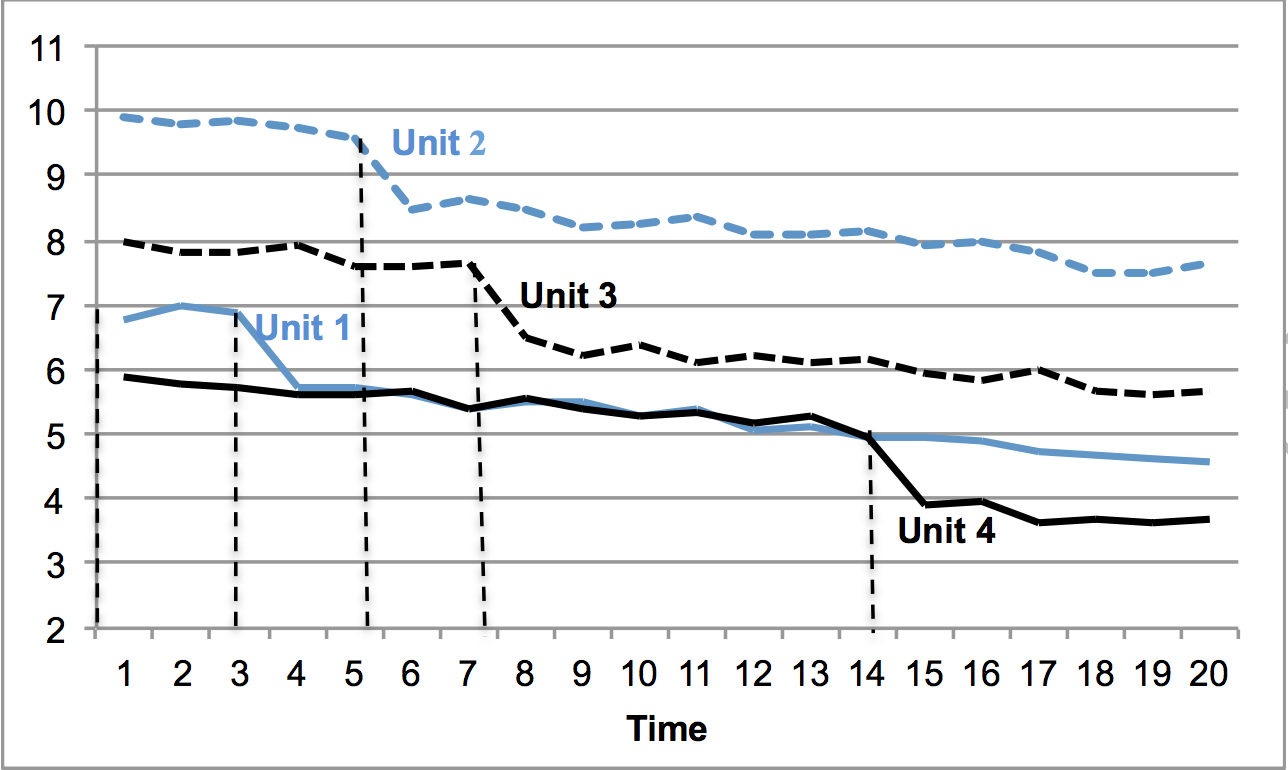
\includegraphics[width=0.7\textwidth,height=\textheight]{"images/PanelRollout.png"}
\caption{Staggered roll out}
\end{figure}

Unit 1 is treated at time 3, unit 2 at time 5, unit 3 at time 7, etc.

Untreated units at time \(t\) serve as the control group for the units
that are being treated at time \(t\).
\end{frame}

\begin{frame}{Generalized DID: Staggered events}
\protect\hypertarget{generalized-did-staggered-events-2}{}
In a regression framework, we would estimate a two-way FE DID,

\[
y_{it}=\beta_0+\beta D_{it}+\gamma_i+\phi_t+u_{it}
\]

The key assumption:

\begin{itemize}
\item
  changes in the control group are a good counterfactual for the change
  in the treatment group
\item
  tests of these assumptions are very similar to the methods we have
  already discussed.
\end{itemize}

The main difference:

\begin{itemize}
\item
  treatment does not happen at a fixed point in time.
\item
  often need to generate a new set of ``relative to event time''
  indicators that are centered around the treatment time of a particular
  unit.
\end{itemize}
\end{frame}

\begin{frame}{Staggered events: WARNING}
\protect\hypertarget{staggered-events-warning}{}
Our understanding of staggered event DID estimations is evolving.

Several recent new papers reassessing these estimation strategies:

\begin{itemize}
\tightlist
\item
  Goodman-Bacon (2018, 2019):

  \begin{itemize}
  \item
    This ``general'' DD estimator is a weighted average of all possible
    two-group/two-period DD estimators in the data: treated units act as
    both controls and treatment depending on the situation
  \item
    How the weighting is done is not clearly theoretically justified
  \item
    Estimates are potentially biased when effects change over time.
  \end{itemize}
\end{itemize}

Exercise caution when using this type of approach as our understanding
of these estimators, and how to correct for their problems is rapidly
evolving.
\end{frame}

\end{document}
